\documentclass[12pt,a4paper,oneside]{article}
\usepackage[QX]{polski}

\usepackage[utf8]{inputenc}
\usepackage{latexsym}
\usepackage{tgpagella}
\usepackage{lmodern}
\usepackage{amsmath,amsthm,amsfonts,amssymb,alltt}
\usepackage{epsfig}
\usepackage{pdflscape}
\usepackage{caption}
\usepackage{indentfirst}
\usepackage{float}
%\usepackage{showkeys}
\bibliographystyle{plabbrv}


\usepackage{color}
\usepackage[polish]{babel}
\usepackage{datetime2}
\usepackage[x11names,dvipsnames,table]{xcolor}
\usepackage{hyperref}
\hypersetup{
pdfauthor={Roman Czapla, Olaf Bar},
colorlinks=True,
linkcolor=darkgray,  % color of internal links (change box color with linkbordercolor)
citecolor=BrickRed,  % color of links to bibliography
filecolor=Magenta,   % color of file links
urlcolor=BlueViolet}	%%pdfpagemode=FullScreen}

% diagramy, grafy itp.
\usepackage{tikz}
\usetikzlibrary{positioning}
\usetikzlibrary{arrows}
\usetikzlibrary{arrows.meta}
\usetikzlibrary{chains,fit,shapes,calc}
\tikzset{main node/.style={circle,fill=blue!20,draw,minimum size=1cm,inner sep=0pt}}

% algorytmy
\usepackage[linesnumbered,lined,commentsnumbered]{algorithm2e}
\SetKwFor{ForEach}{for each}{do}{end for}%
\SetKwFor{ForAll}{for all}{do}{end for}%
\newenvironment{myalgorithm}
{\rule{\textwidth}{0.5mm}\\\SetAlCapSty{}\SetAlgoNoEnd\SetAlgoNoLine\begin{algorithm}}{\end{algorithm}\rule{\textwidth}{0.5mm}}


%---------------------
\overfullrule=2mm
\pagestyle{plain}
\textwidth=15cm \textheight=685pt \topmargin=-25pt \linespread{1.3} 
\setlength{\parskip}{0pt}
\setlength\arraycolsep{2pt}
\oddsidemargin =0.9cm
\evensidemargin =-0.1cm

\captionsetup{width=.95\linewidth, justification=centering}
%---------------------




\newtheorem{tw}{Twierdzenie}[section]
\newtheorem{lem}[tw]{Lemat}
\newtheorem{co}[tw]{Wniosek}
\newtheorem{prop}[tw]{Stwierdzenie}
\theoremstyle{definition}
\newtheorem{ex}{Przykład}
\newtheorem{re}[tw]{Uwaga}
\newtheorem{de}{Definicja}[section]



\newcommand{\bC}{{\mathbb C}}
\newcommand{\bR}{{\mathbb R}}
\newcommand{\bZ}{{\mathbb Z}}
\newcommand{\bQ}{{\mathbb Q}}
\newcommand{\bN}{{\mathbb N}}
\newcommand{\captionT}[1]{\caption{\textsc{\footnotesize{#1}}}}
\renewcommand\figurename{Rys.}

\numberwithin{equation}{section}
\renewcommand{\thefootnote}{\arabic{footnote})}
%\renewcommand{\thefootnote}{\alph{footnote})}



\begin{document}

% --------------------------------------------
% Strona tytułowa
% --------------------------------------------

\thispagestyle{empty}
\begin{titlepage}
\begin{center}\Large
Uniwersytet Komisji Edukacji Narodowej w Krakowie\\
\large
Instytut Bezpieczeństwa i Informatyki\\
\vskip 10pt
\end{center}
\begin{center}
\centering 
\includegraphics[width=1.0\columnwidth]{images/logo.png}
\end{center}

\begin{center}
 {\bf \fontsize{14pt}{14pt}\selectfont PROJEKT INŻYNIERSKI \\ RAPORT Z REALIZACJI PROJEKTU\\
 }
 {\fontsize{12pt}{12pt} raport z okres: dd.mm.rrrr - dd.mm.rrrr}
\end{center}
\vskip 5pt
\begin{center}
 {\bf \fontsize{22pt}{22pt}\selectfont System rekomendacji produktów. Tworzenie algorytmu rekomendacyjnego na
 podstawie preferencji użytkowników – aplikacja przeglądarkowa}
\end{center}

\begin{center}
 {\fontsize{12pt}{12pt}\selectfont wykonany przez: }
\end{center}
\begin{center}
 {\bf\fontsize{16pt}{16pt}\selectfont Krzysztof Bielkiewicz}\\
 {\fontsize{12pt}{12pt}\selectfont Nr albumu: 156791 \\\&\\}
 {\bf\fontsize{16pt}{16pt}\selectfont Anna Nowak}\\
 {\fontsize{12pt}{12pt}\selectfont Nr albumu: XXXXX\\\&\\}
 {\bf\fontsize{16pt}{16pt}\selectfont Karol Woźniak}\\
 {\fontsize{12pt}{12pt}\selectfont Nr albumu: XXXXX}
\end{center}
\begin{center}
 {\fontsize{12pt}{12pt}\selectfont pod opieką:}\\
 {\bf\fontsize{12pt}{12pt}\selectfont dr hab. inż. Mateusz Muchacki, prof. UKEN}
\end{center}

%\mbox{}
\vspace*{\fill}
%\vskip 50pt
\begin{center}
\large
Kraków \the\year\\
(ostatnia aktualizacja: \DTMcurrenttime,\;\today)
\end{center}
\end{titlepage}
\setcounter{page}{0} 
\newpage\null\thispagestyle{empty}
%\setcounter{page}{0} 
%\newpage
%\thispagestyle{empty}

\tableofcontents


\newpage

\section{Informacja na temat postępów prac nad projektem}

\subsection{Zespół projektowy}
\textit{Lista osób tworzących zespół projektowy wraz z danymi kontaktowi (e-mail).}
    \paragraph{Grzegorz Golonka}
    \begin{itemize}
        \item E-mail:
    \end{itemize}
    \paragraph{Krzysztof Bielkiewicz}
    \begin{itemize}
        \item E-mail:  krzysztof.bielkiewicz@student.up.krakow.pl
    \end{itemize}
    \paragraph{Maciej Faber}
    \begin{itemize}
        \item E-mail:
    \end{itemize}

\subsection{Zrealizowane zadania}
\textit{Lista zrealizowanych prac z podziałem na członków zespołu projektowego.}
\paragraph{Krzysztof Bielkiewicz}
\begin{itemize}
\item Zadanie 1. Stworzenie nagłówka dla aplikacji (\hyperref[1.3.1]{sekcja 1.3.1})
\item Zadanie 2. Stworzenie strony startowej (\hyperref[1.3.2]{sekcja 1.3.2})
\item Zadanie 3. Opcja wyszukiwania po słowach kluczowych (\hyperref[1.3.3]{sekcja 1.3.3})
\item Zadanie 4. Opcja wyszukiwania po kategoriach (\hyperref[1.3.4]{sekcja 1.3.4})
\item Zadanie 5. Stworzenie strony z ulubionymi produktami (\hyperref[1.3.5]{sekcja 1.3.5})
\item Zadanie 6. Stworzenie strony profilu z opcją edycji (\hyperref[1.3.6]{sekcja 1.3.6})
\item Zadanie 7. Oprawa graficzna dla strony dodania adresu dostawy (\hyperref[1.3.7]{sekcja 1.3.7})
\item Zadanie 8. Oprawa graficzna koszyka (\hyperref[1.3.8]{sekcja 1.3.8})
\item Zadanie 9. Oprawa graficzna wyboru adresu dostawy (\hyperref[1.3.9]{sekcja 1.3.9})
\item Zadanie 10. Oprawa graficzna dla metod płatności (\hyperref[1.3.10]{sekcja 1.3.10})
\item Zadanie 11. Oprawa graficzna szczegółów zamówienia (\hyperref[1.3.11]{sekcja 1.3.11})
\item Zadanie 12. Oprawa graficzna dla listy zamówień (\hyperref[1.3.12]{sekcja 1.3.12})
\item Zadanie 13. Wyświetlanie produktów z bazy danych (\hyperref[1.3.13]{sekcja 1.3.13})
\item Zadanie 14. Funckja dodawania produktów do ulubionych (\hyperref[1.3.14]{sekcja 1.3.14})
\item Zadanie 15. Paginacja produktów na stronach (\hyperref[1.3.15]{sekcja 1.3.15})
\item Zadanie 16. Oprawa graficzna szczegółów produktu (\hyperref[1.3.16]{sekcja 1.3.16})
\item Zadanie 17. Custom errory i oprawa graficzna rejestracji (\hyperref[1.3.17]{sekcja 1.3.17})
\item Zadanie 18. Custom errory i oprawa graficzna loginu (\hyperref[1.3.18]{sekcja 1.3.18})
\end{itemize}
\paragraph{Anna Nowak}
\begin{itemize}
\item zadanie nr 1 (sekcja 1.3.n+1)
\item zadanie nr 2 (sekcja 1.3.n+2)
\item \dots
\item zadanie nr m (sekcja 1.3.n+m)
\end{itemize}
\paragraph{Karol Woźniak}
\begin{itemize}
\item zadanie nr 1 (sekcja 1.3.m+1)
\item zadanie nr 2 (sekcja 1.3.m+2)
\item \dots
\item zadanie nr k (sekcja 1.3.m+k)

\end{itemize}

\subsection {Opis zrealizowanych prac}
\subsubsection{Krzysztof Bielkiewicz: Stworzenie nagłówka dla aplikacji}
\label{1.3.1}
\textit{Responsywny nagłówek dla całej aplikacji, zawierający:}
\begin{itemize}
    \item Nazwe aplikacji, funkcje wyszukiwania
    \item Przycisk z wyborem kategorii i przekierowania do produktów z wybranej kategorii
    \item Przyciski przekierowania do strony z Ulubione i Koszyka
    \item Przycisk Profile pokazujący przyciski przekierowujące do:
        \begin{itemize}
            \item Edycji profilu, Dodania adresu
            \item Wiadomości, Szczegółów zamówienia
            \item Wylogowania
        \end{itemize}
\end{itemize}

\begin{figure}[H]
    \centering
    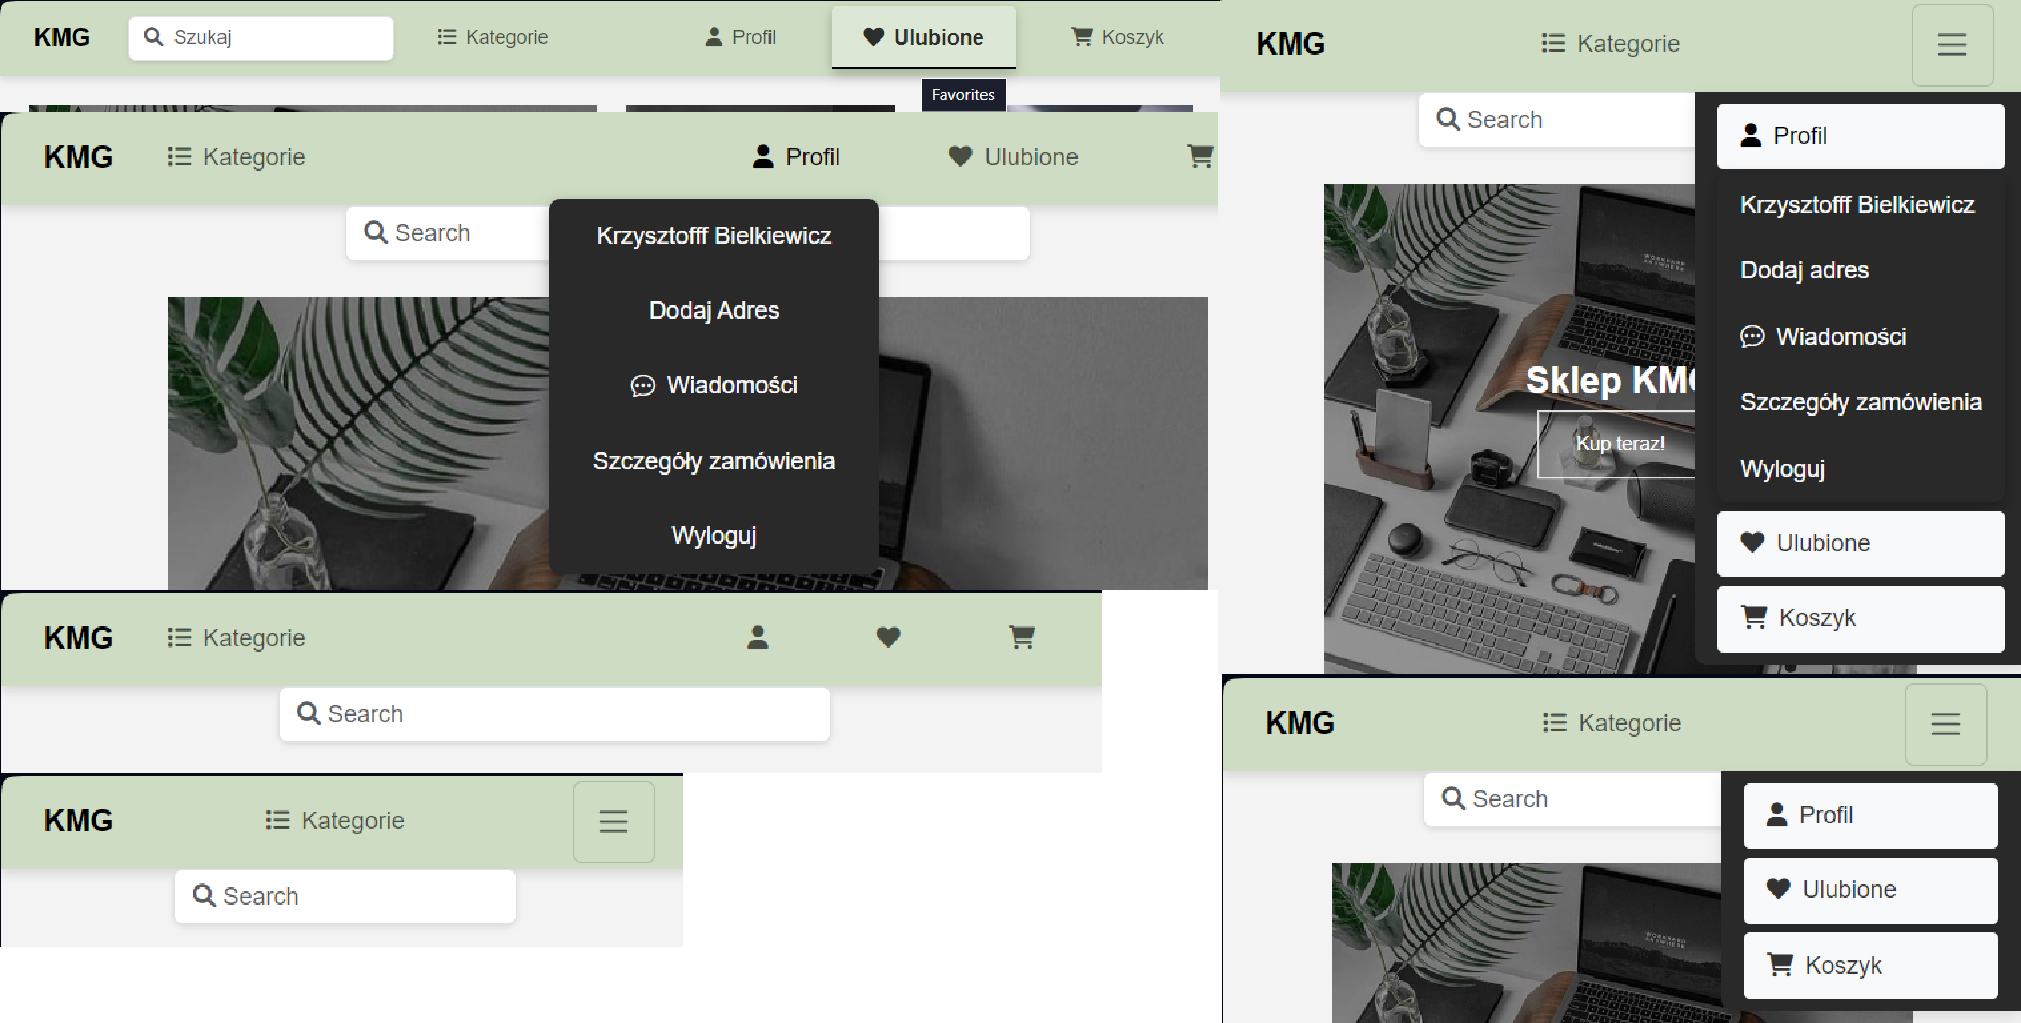
\includegraphics[width=0.9\columnwidth]{images/krzysztofBImages/header.png}
    \caption{Nagłówek z przyciskami}
    \label{header}
\end{figure}

\begin{figure}[H]
    \centering
    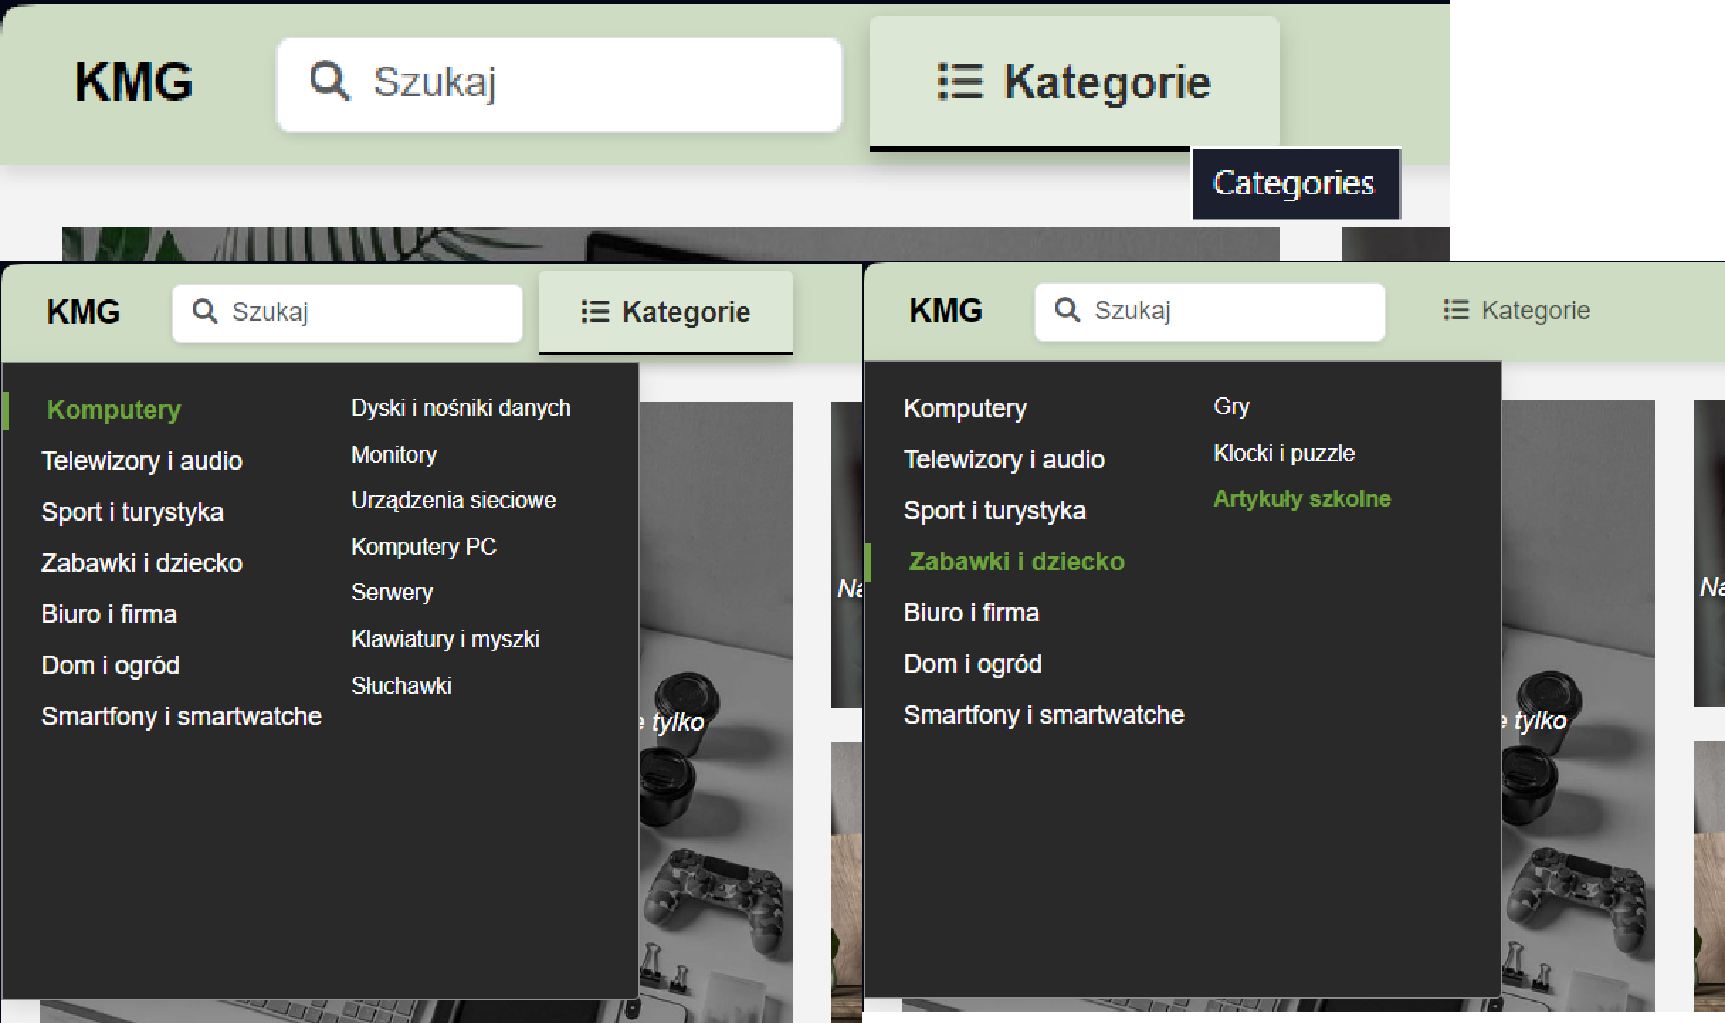
\includegraphics[width=0.9\columnwidth]{images/krzysztofBImages/header-categories.png}
    \caption{Wybór kategorii w nagłówku}
    \label{header-categories}
\end{figure}


\subsubsection{Krzysztof Bielkiewicz: Stworzenie strony startowej}
\label{1.3.2}
\textit{Responsywna strona startowa zawierająca:}
    \begin{itemize}
        \item Główny baner z przekierowaniami do poszczególnych kategorii
        \item Interaktywny slider wyświetlający polecane produkty oraz drugi co wyświetla polubione produkty
        \item Stopka
    \end{itemize}

    \begin{figure}[H]
        \centering
        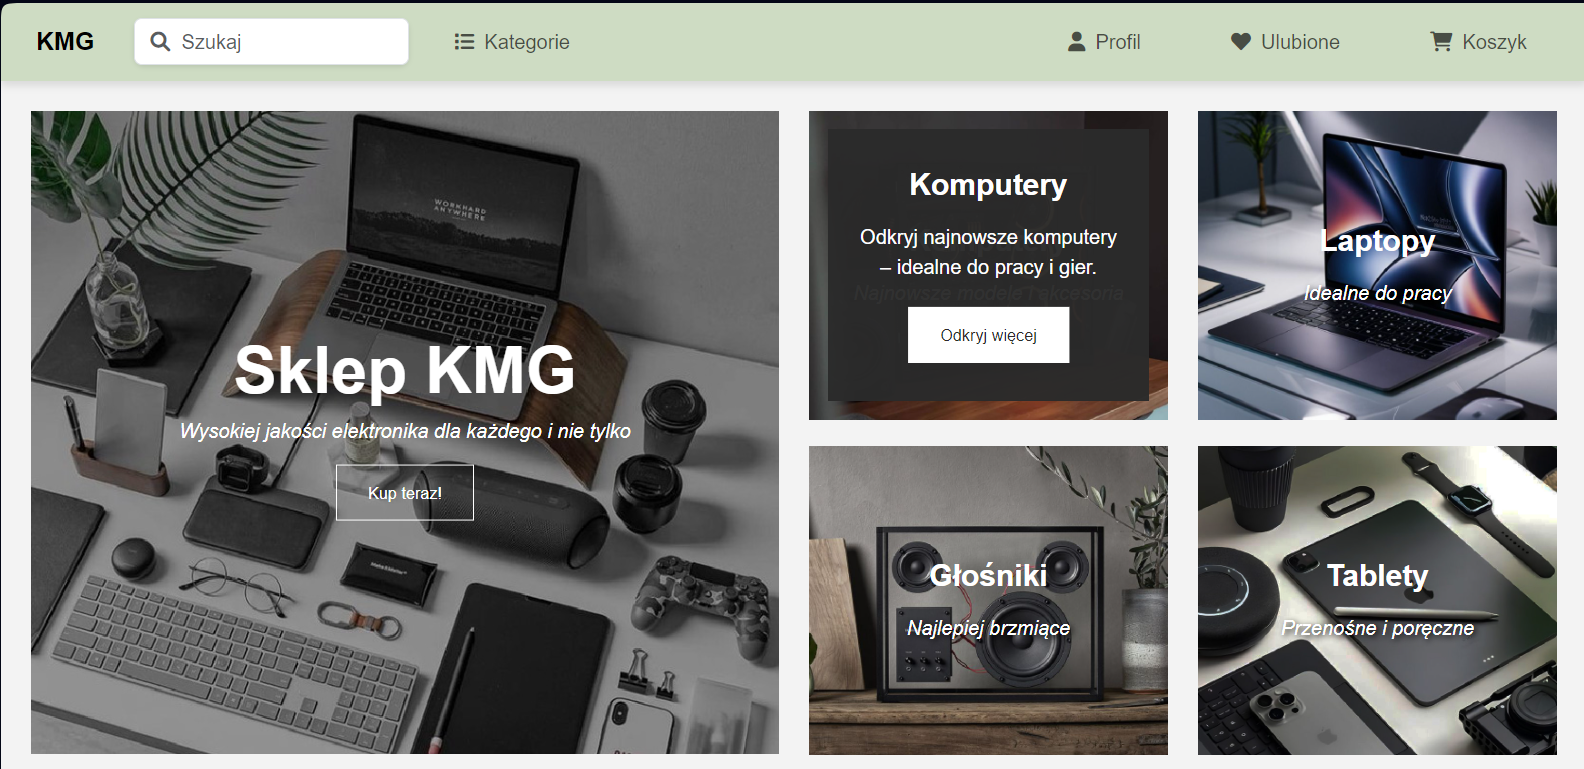
\includegraphics[width=0.8\columnwidth]{images/krzysztofBImages/main-banner.png}
        \caption{Główny banner}
        \label{main-banner}
    \end{figure}

    \begin{figure}[H]
        \centering
        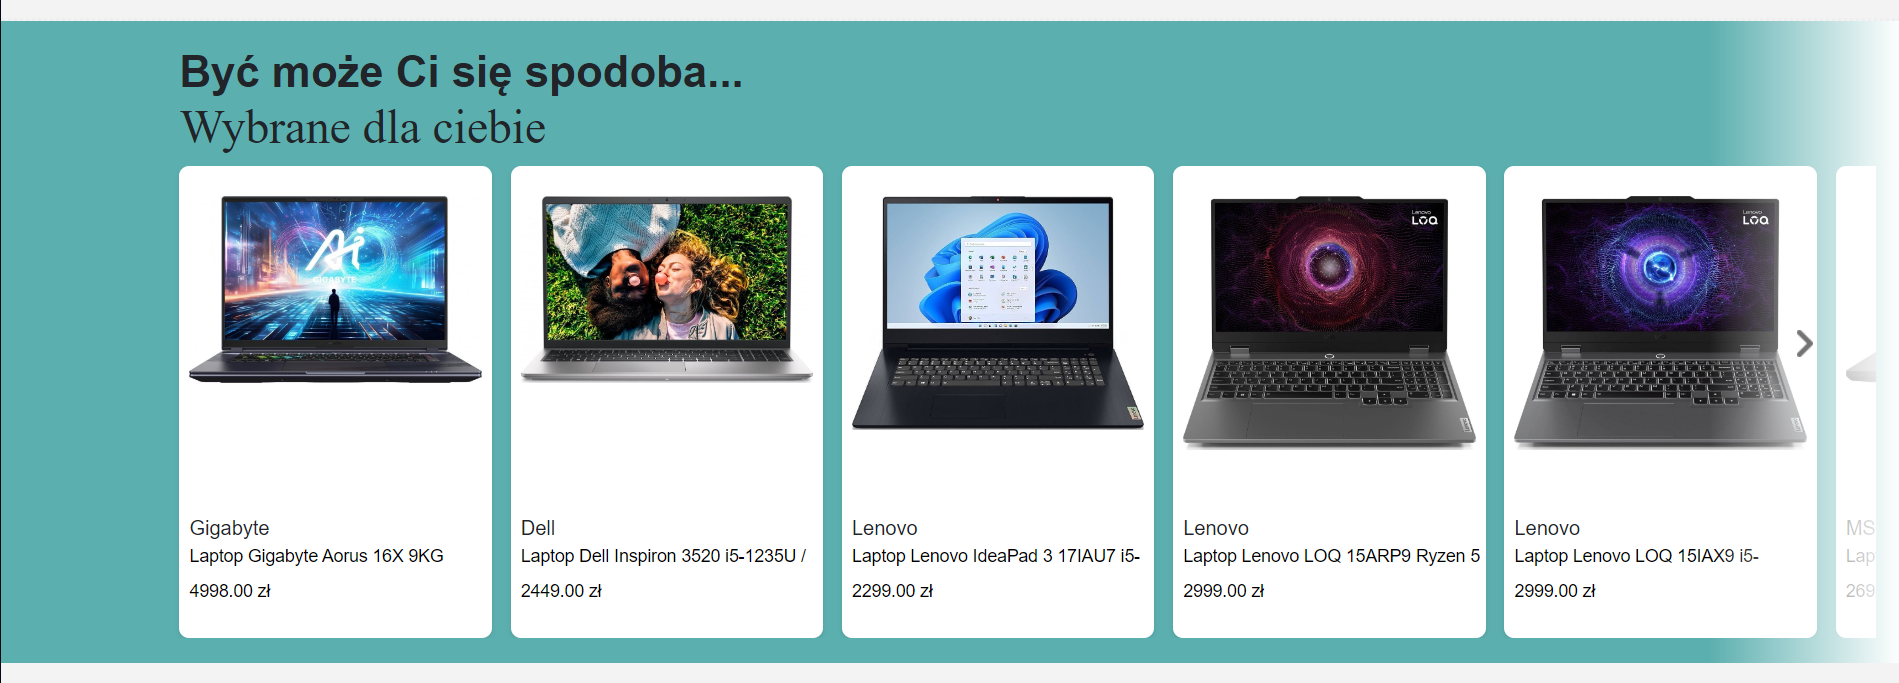
\includegraphics[width=0.7\columnwidth]{images/krzysztofBImages/slider-polecane.png}
        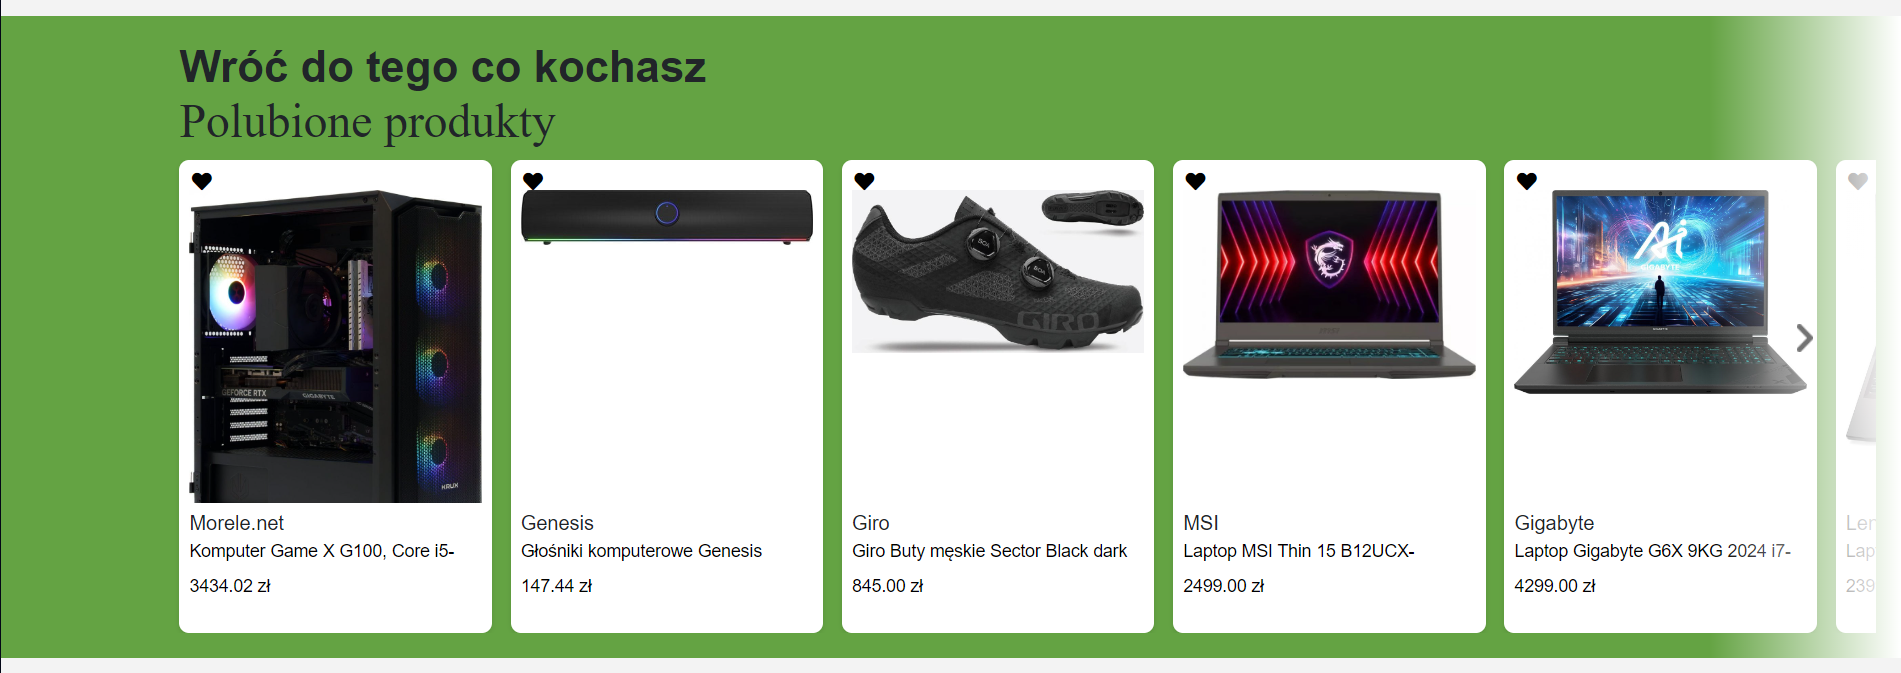
\includegraphics[width=0.7\columnwidth]{images/krzysztofBImages/slider-ulubione.png}
        \caption{Slider z polecanymi i polubionymi}
        \label{Slider}
    \end{figure}

    \begin{figure}[H]
        \centering
        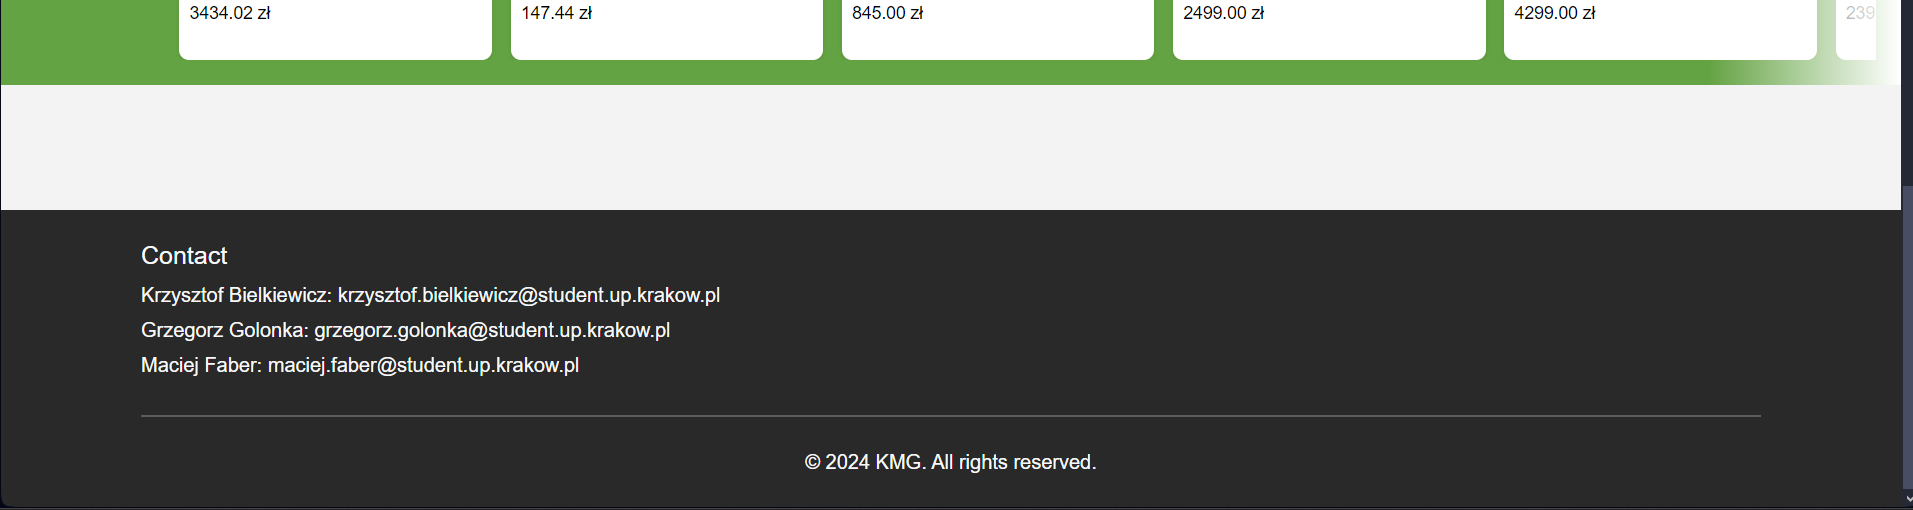
\includegraphics[width=0.7\columnwidth]{images/krzysztofBImages/footer.png}
        \caption{Stopka}
        \label{Stopka}
    \end{figure}


\subsubsection{Krzysztof Bielkiewicz: Opcja wyszukiwania po słowach kluczowych}
\label{1.3.3}
\textit{Implementacja w backend wyszukiwania po słowach wpisanych w rubryce 'Szukaj'
oraz strona wyświetlająca wynik wyszukiwania i jej oprawa graficzna.}
\begin{figure}[H]
    \centering
    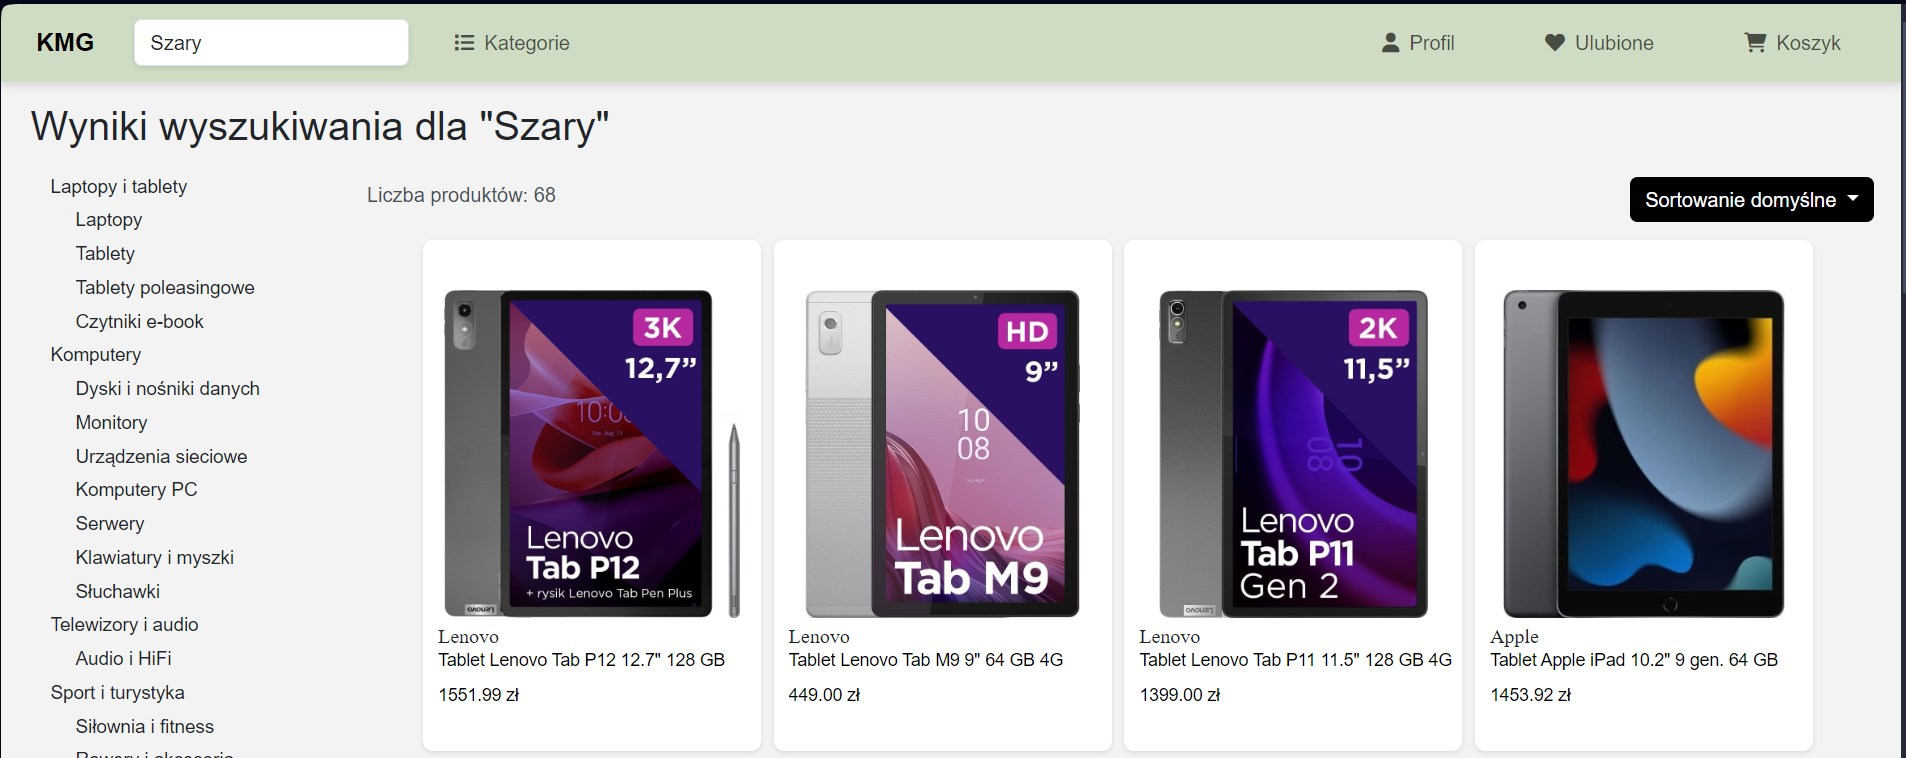
\includegraphics[width=0.8\columnwidth]{images/krzysztofBImages/wyszukiwanie.png}
    \caption{Wynik wyszukiwania}
    \label{search-value}
\end{figure}

    
\subsubsection{Krzysztof Bielkiewicz: Opcja wyszukiwania po kategoriach}
\label{1.3.4}
    \textit{Zaimplementowana w backend opcja wyszukiwania po kategoriach
     oraz stworzenie w frontend liste kategorii w nagłówku
      oraz liste kategorii po lewej stronie od wyświetlanych produktów w której jest zaznaczona
      aktualnie przeglądana kategoria. Utworzenie strony z wyświetlanymi produktami z wybranej kategorii.}
    \begin{center}
        \hyperref[header-categories]{Zdjęcie wyszukiwania po kategoriach w nagłówku}
    \end{center}

    \begin{figure}[H]
        \centering
        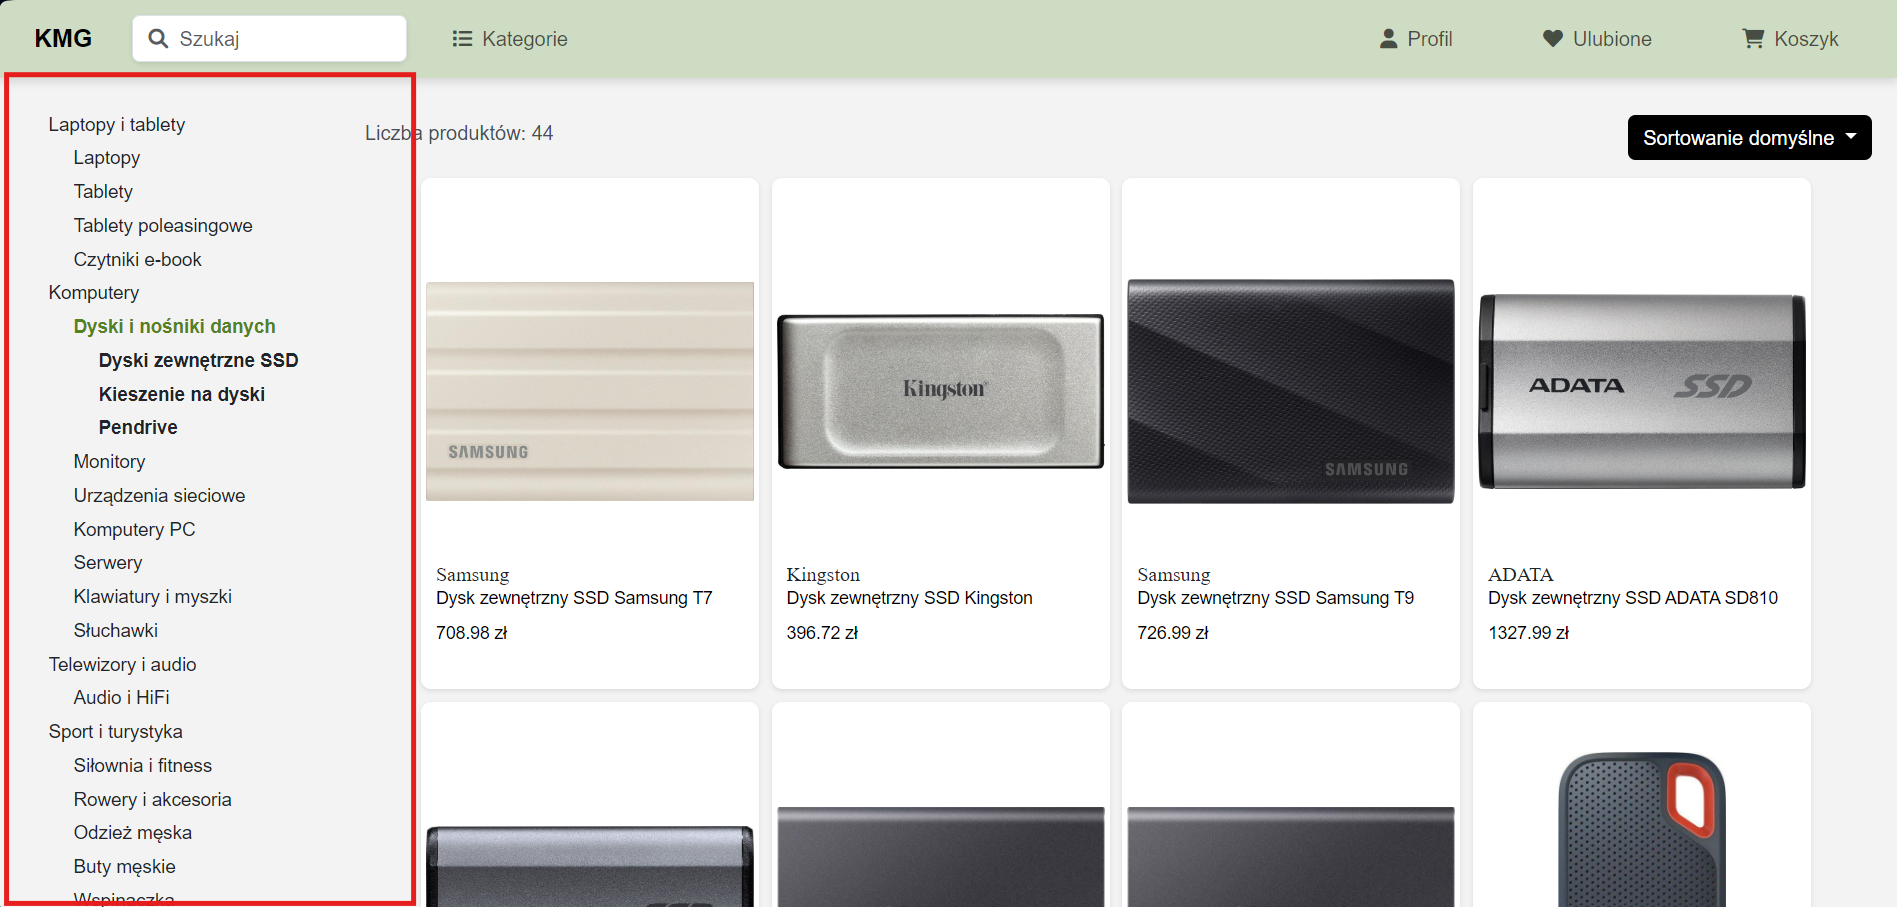
\includegraphics[width=0.8\columnwidth]{images/krzysztofBImages/lewe-kategorie.png}
        \caption{Kategorie po lewej stronie na stronie z produktami z wybranej kategorii}
        \label{left-categories}
    \end{figure}


\subsubsection{Krzysztof Bielkiewicz: Stworzenie strony z ulubionymi produktami}
\label{1.3.5}
\textit{Strona wyświetlająca produkty polubione przez użytkownika/lub w danej sesji.}

\begin{figure}[H]
    \centering
    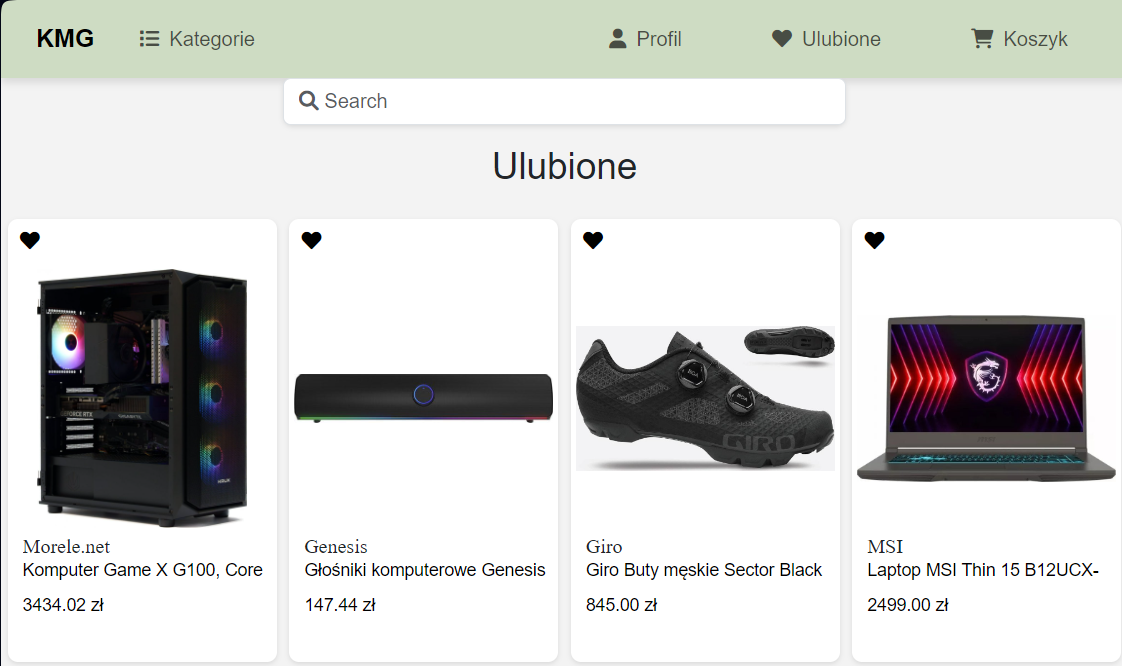
\includegraphics[width=0.8\columnwidth]{images/krzysztofBImages/strona-ulubione.png}
    \caption{Strona z polubionymi produktami}
    \label{strona-ulubione}
\end{figure}

\subsubsection{Krzysztof Bielkiewicz: Stworzenie strony profilu z opcją edycji}
\label{1.3.6}
\textit{Stworzenie responsywnej strony w backend i frontend do edycji danych z modelu User.
Umożliwia edycje podstawych danych jak e-mail, imię, date urodzenia, itp.
Oraz umożliwia zmianę hasła.}

\begin{figure}[H]
    \centering
    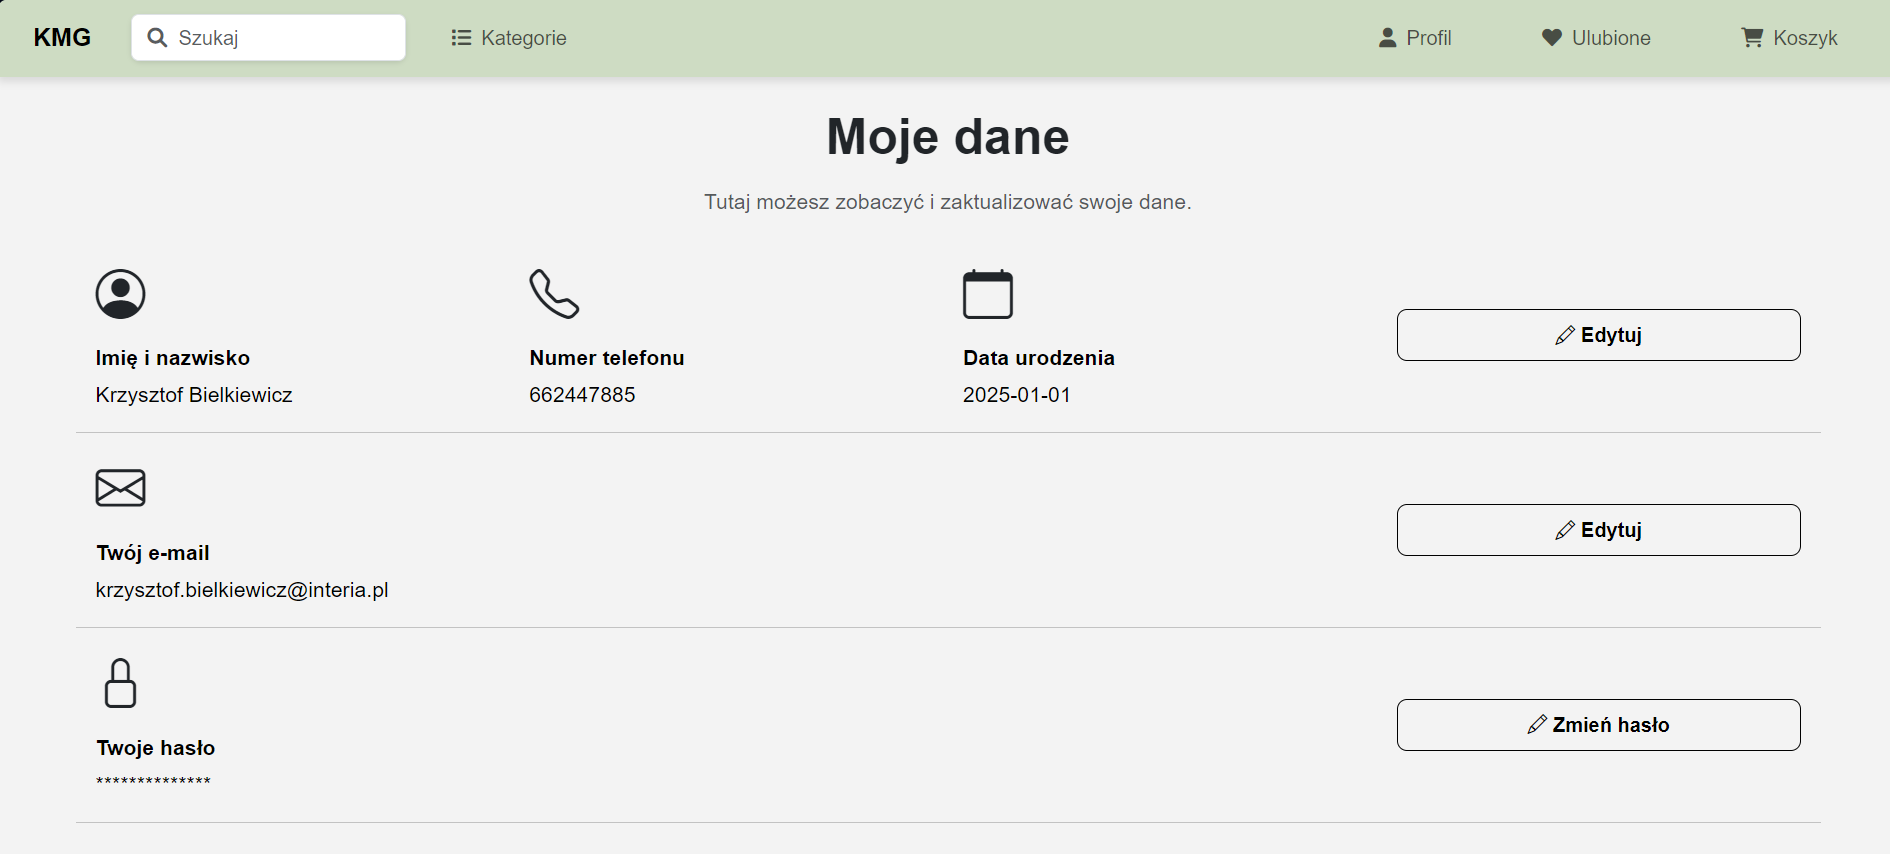
\includegraphics[width=0.9\columnwidth]{images/krzysztofBImages/profil/strona-edycji-profilu.png}
    \caption{Strona z polami do edycji profilu}
    \label{strona-edycji-profilu}
\end{figure}

\begin{figure}[H]
    \centering
    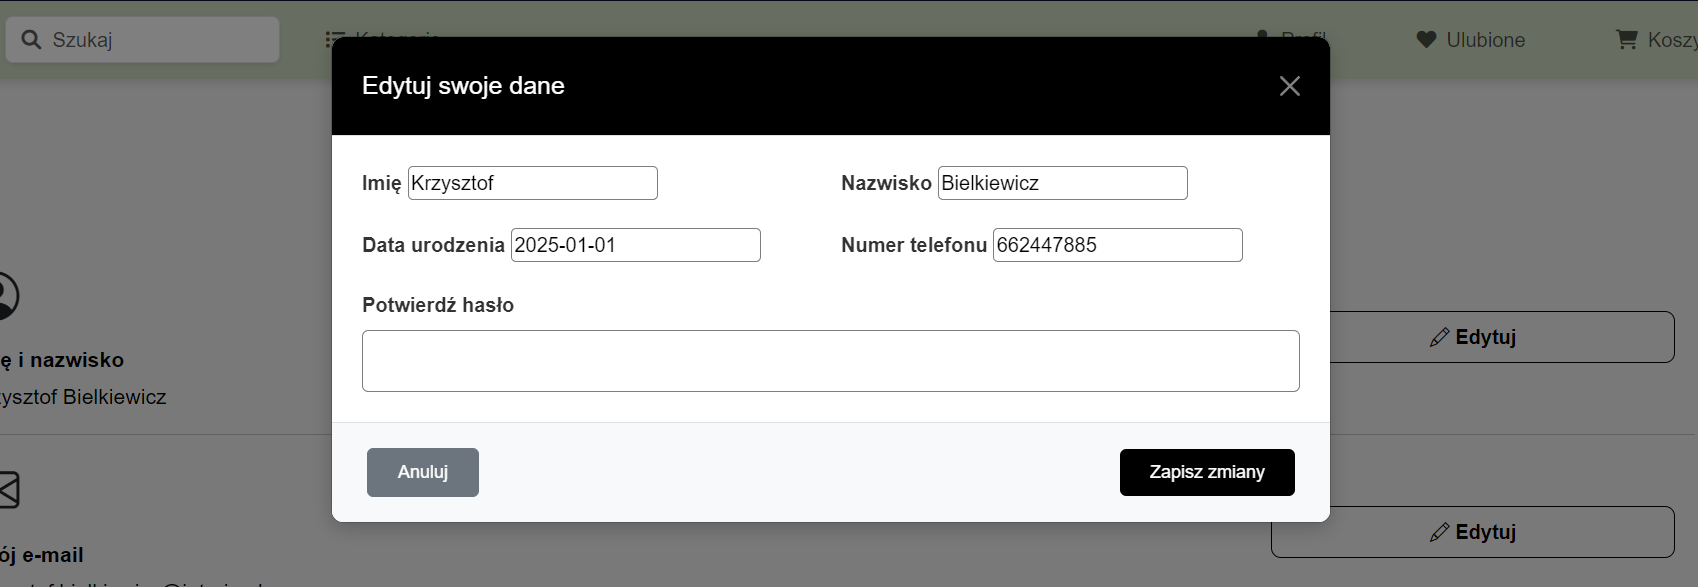
\includegraphics[width=0.9\columnwidth]{images/krzysztofBImages/profil/edycja-danych.png}
    \caption{Formularz edytowania podstawowych danych}
    \label{edycja-danych}
\end{figure}

\begin{figure}[H]
    \centering
    \includegraphics[width=0.9\columnwidth]{images/krzysztofBImages/profil/zmiana-hasła.png}
    \caption{Formularz zmiany hasła}
    \label{zmiana-hasła}
\end{figure}

\begin{figure}[H]
    \centering
    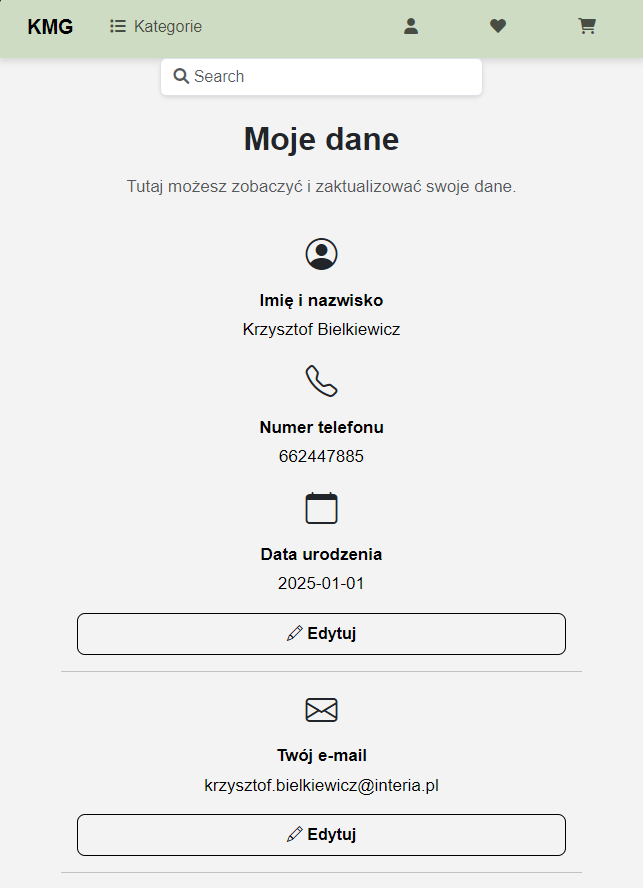
\includegraphics[width=0.5\columnwidth]{images/krzysztofBImages/profil/responywna-strona-profilu.png}
    \caption{Responywna strona edycji profilu}
    \label{responywna-strona-profilu}
\end{figure}

\subsubsection{Krzysztof Bielkiewicz: Oprawa graficzna strony adresu dostawy}
\label{1.3.7}
\textit{Utworzenie oprawy graficznej dla strony dodania adresu dostawy.}
\begin{figure}[H]
    \centering
    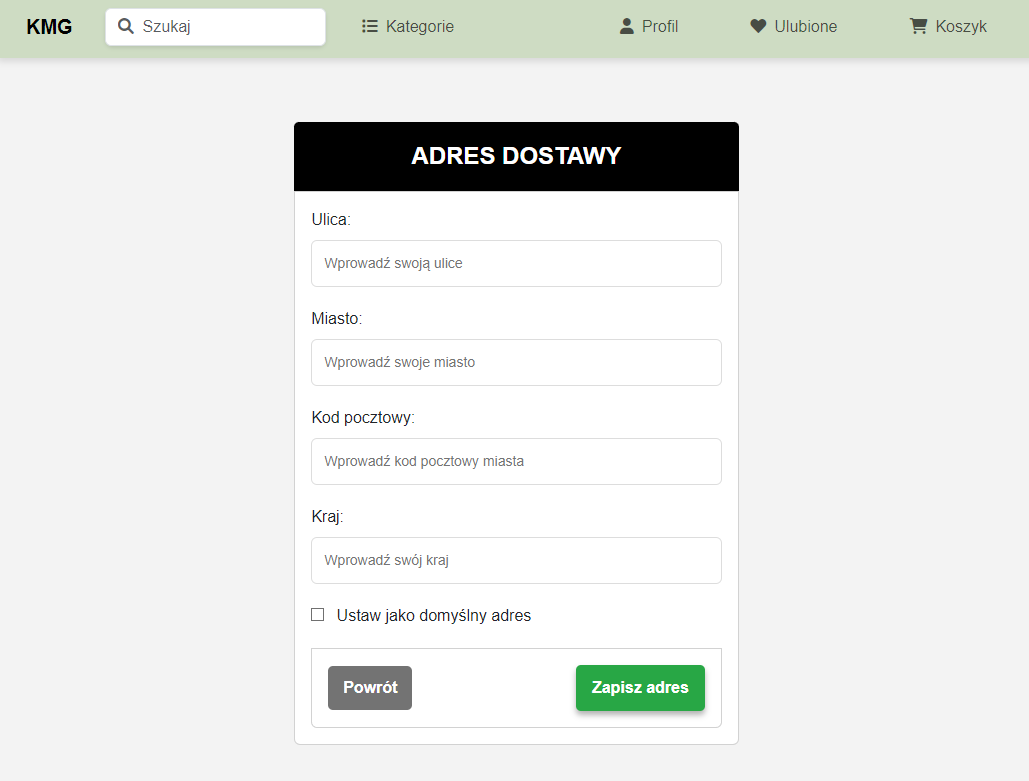
\includegraphics[width=0.8\columnwidth]{images/krzysztofBImages/strona-dodaj-adres.png}
    \caption{Strona z formularzem dodania adresu dostawy}
    \label{dodaj-adres}
\end{figure}

\subsubsection{Krzysztof Bielkiewicz: Oprawa graficzna koszyka}
\label{1.3.8}
\textit{Utworzenie oprawy graficznej dla koszyka i jej responywność.}
\begin{figure}[H]
    \centering
    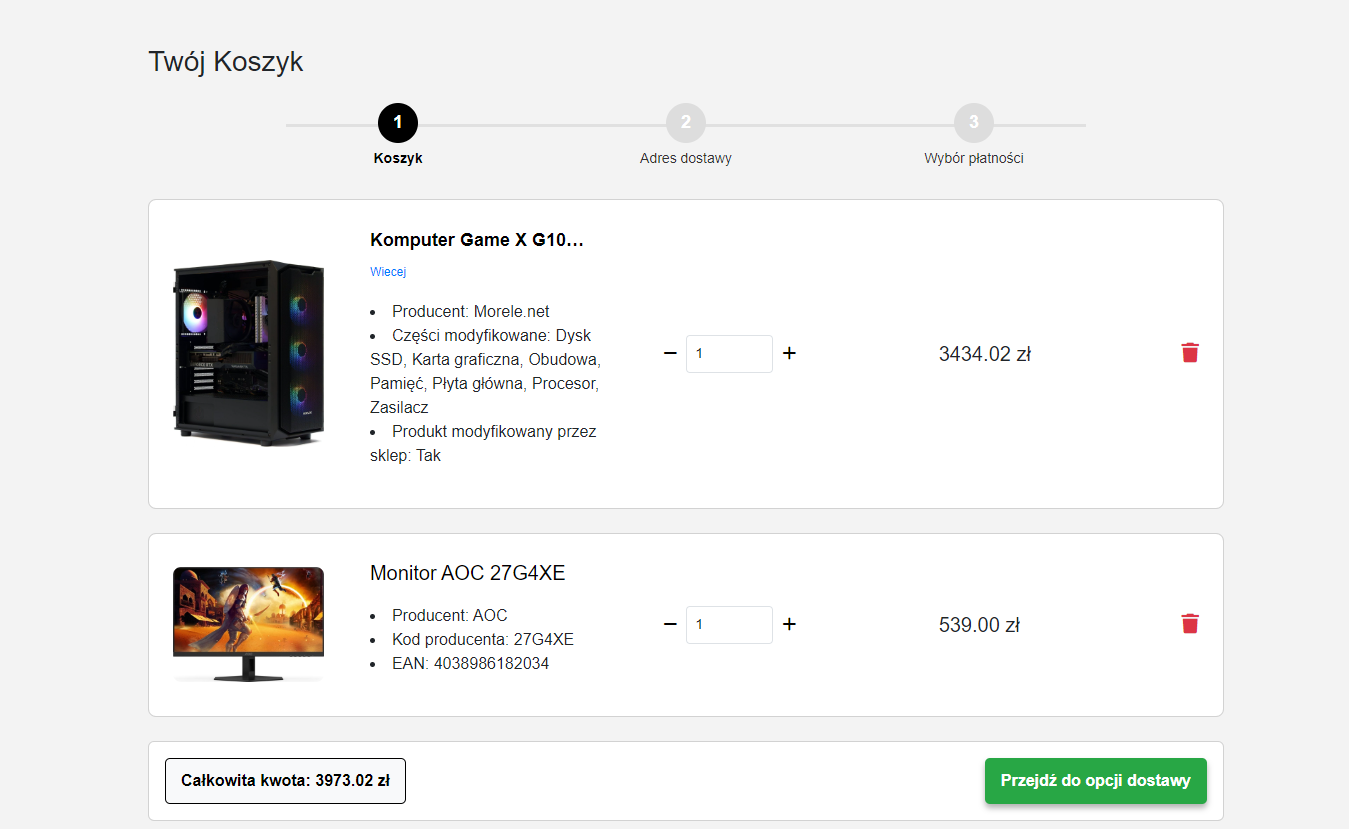
\includegraphics[width=0.8\columnwidth]{images/krzysztofBImages/cart/cart-step1.png}
    \caption{Strona koszyka}
    \label{cart-step1}
\end{figure}

\begin{figure}[H]
    \centering
    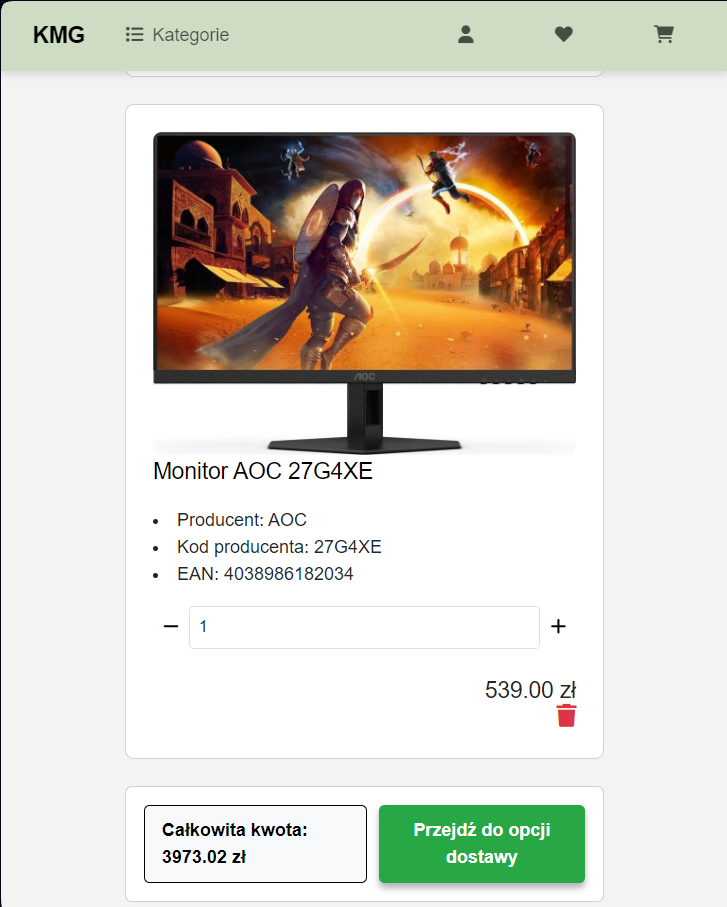
\includegraphics[width=0.5\columnwidth]{images/krzysztofBImages/cart/cart-step1-respo.png}
    \caption{Strona koszyka - responsywna}
    \label{cart-step1-respo}
\end{figure}

\subsubsection{Krzysztof Bielkiewicz: Oprawa graficzna wyboru adresu dostawy}
\label{1.3.9}
\textit{Utworzenie oprawy graficznej dla wyboru adresu dostawy.}
\begin{figure}[H]
    \centering
    \includegraphics[width=0.8\columnwidth]{images/krzysztofBImages/cart/wybór-adresu-dostawy.png}
    \caption{Strona wyboru adresu dostawy}
    \label{płatność-kartą}
\end{figure}

\subsubsection{Krzysztof Bielkiewicz: Oprawa graficzna dla metod płatności}
\label{1.3.10}
\textit{Utworzenie oprawy graficznej metod płatności. }
\begin{figure}[H]
    \centering
    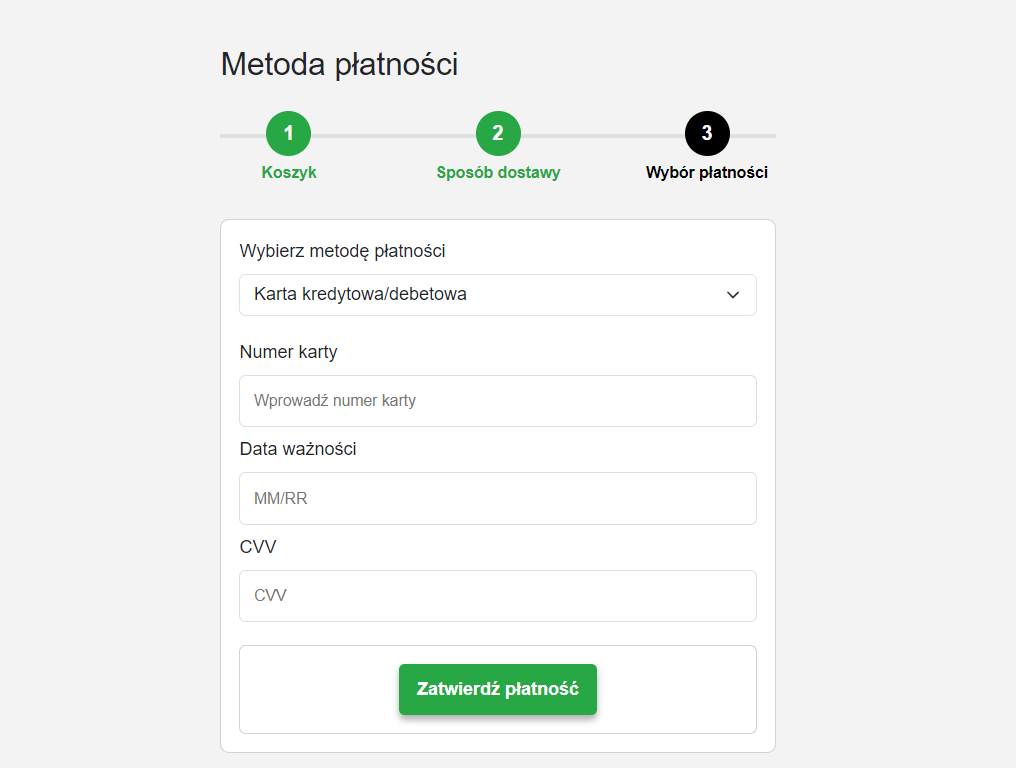
\includegraphics[width=0.8\columnwidth]{images/krzysztofBImages/cart/metody-płatności-karta.png}
    \caption{Metoda płatności kartą}
    \label{płatność-karta}
\end{figure}

\begin{figure}[H]
    \centering
    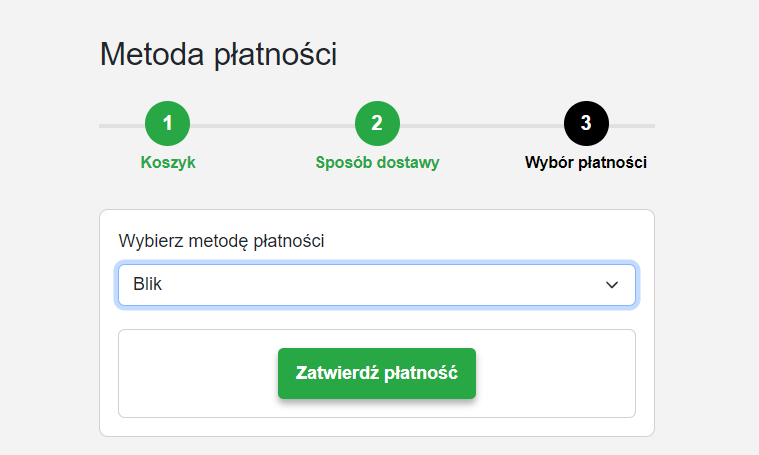
\includegraphics[width=1.0\columnwidth]{images/krzysztofBImages/cart/metody-płatności-blik.png}
    \caption{Metoda płatności blik}
    \label{płatność-blik}
\end{figure}

\begin{figure}[H]
    \centering
    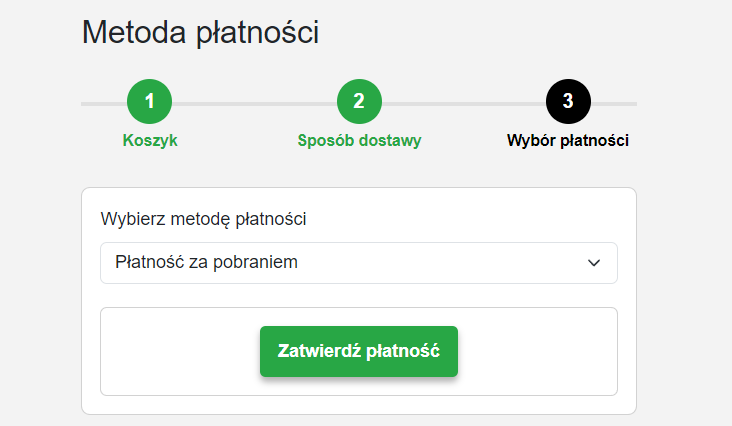
\includegraphics[width=0.8\columnwidth]{images/krzysztofBImages/cart/metody-płatności-za-pobraniem.png}
    \caption{Metoda płatności za pobraniem}
    \label{płatność-zapobraniem}
\end{figure}

\subsubsection{Krzysztof Bielkiewicz: Oprawa graficzna szczegółów zamówienia}
\label{1.3.11}
\textit{Utworzenie oprawy graficznej dla strony ze szegółami zamówienia i jej responywność.}

\begin{figure}[H]
    \centering
    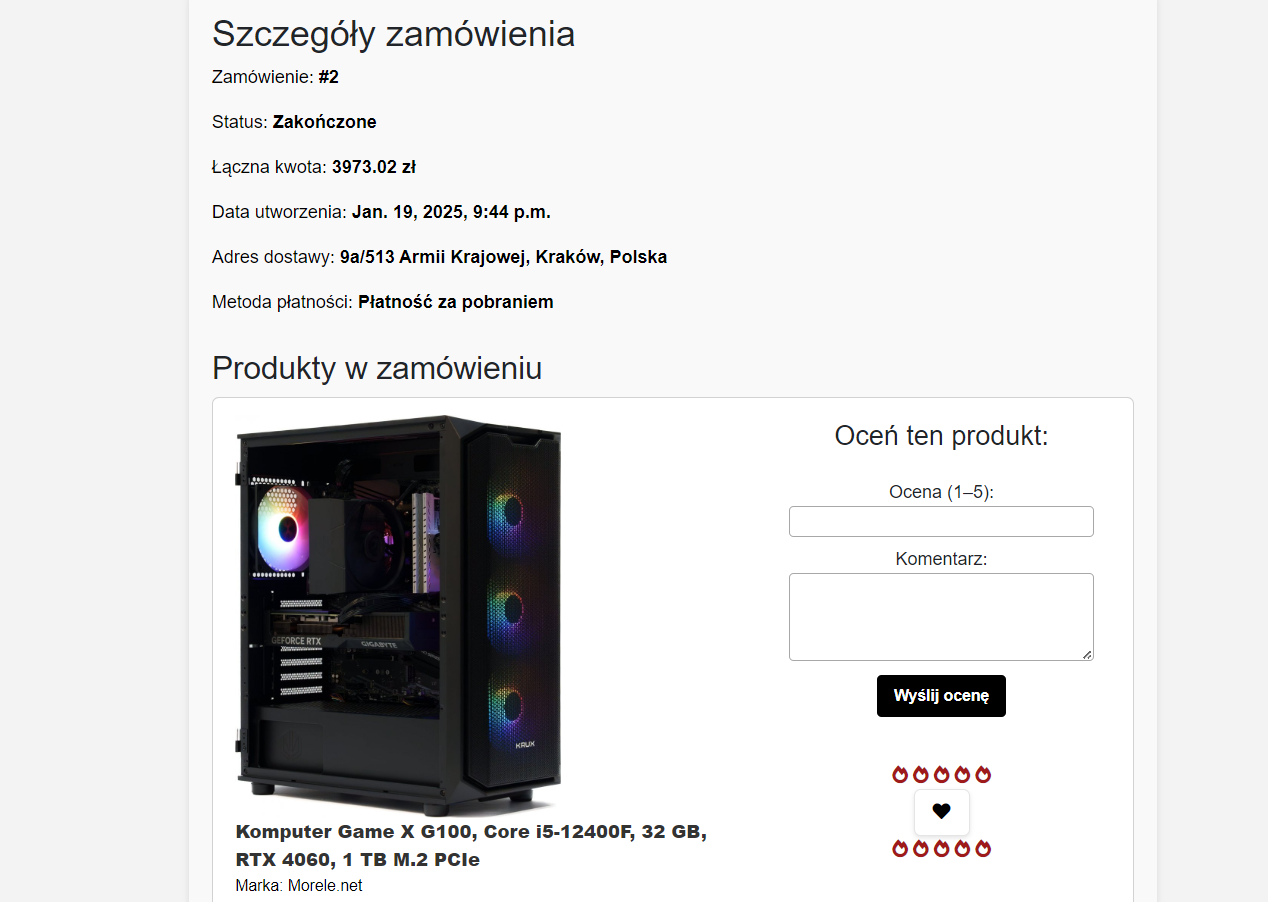
\includegraphics[width=0.8\columnwidth]{images/krzysztofBImages/szczegóły-zamówieniaV1.png}
    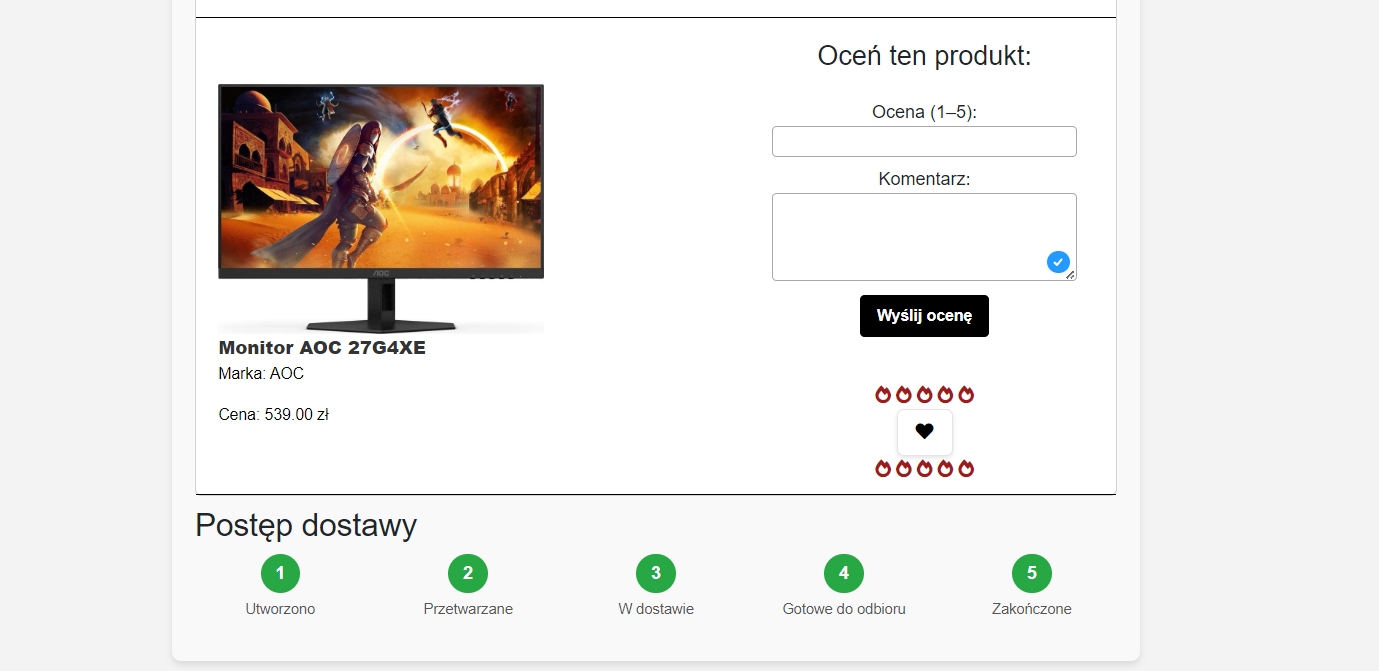
\includegraphics[width=0.8\columnwidth]{images/krzysztofBImages/szczegóły-zamówieniaV2.png}
    \caption{Strona ze szegółami zamówienia}
    \label{szczegóły-zamówienia}
\end{figure}

\begin{figure}[H]
    \centering
    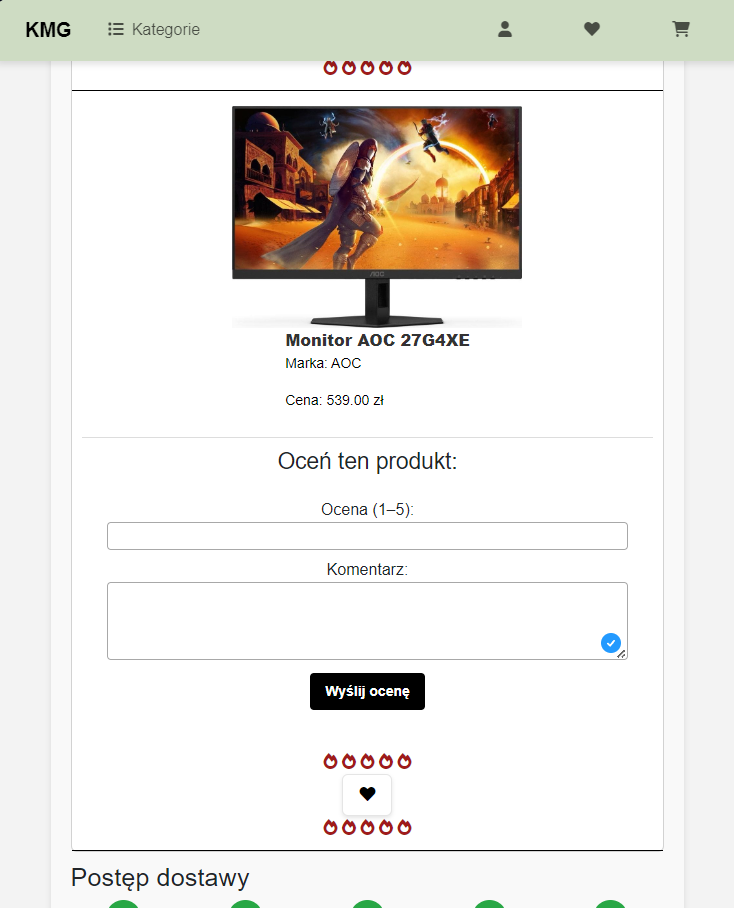
\includegraphics[width=0.5\columnwidth]{images/krzysztofBImages/szczegóły-zamówienia-respo.png}
    \caption{Responywna strona ze szegółami zamówienia}
    \label{szczegóły-zamówienia-respo}
\end{figure}

\subsubsection{Krzysztof Bielkiewicz: Oprawa graficzna dla listy zamówień}
\label{1.3.12}
\textit{Utworzenie oprawy graficznej dla listy zamówień.}

\begin{figure}[H]
    \centering
    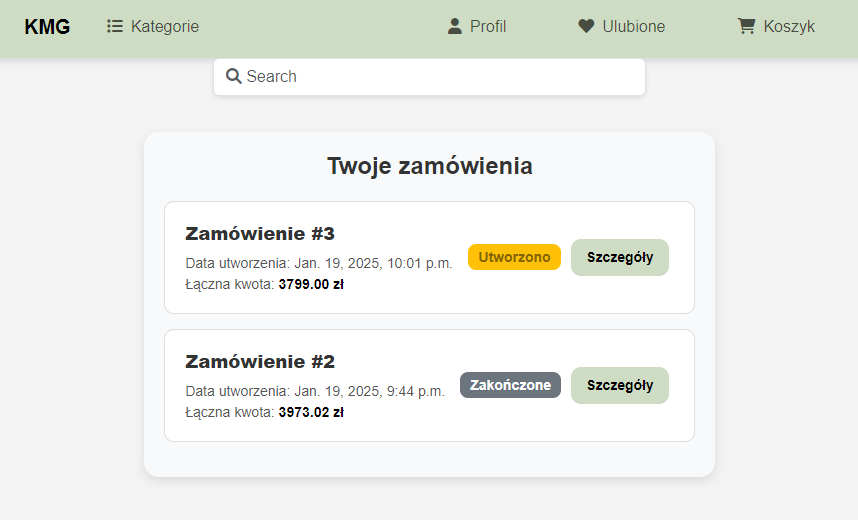
\includegraphics[width=0.8\columnwidth]{images/krzysztofBImages/orders.png}
    \caption{Lista zamówień}
    \label{orders}
\end{figure}


\subsubsection{Krzysztof Bielkiewicz: Wyświetlenie produktów z bazy danych}
\label{1.3.13}
\textit{Utworzenie strony wyświetlającej produkty z podstawowymi danymi: marka, tytuł, cena oraz zdjęcie.
Przyciski polubienia i koszyka dla każdego produktu po najechaniu na dany produkt.
Produkty polubione przez użytkownika mają widoczne serca.
Oprawa graficzna dla wyświetlanych prduktów i przycisków polubienia i dodania do koszyka.}
\begin{figure}[H]
    \centering
    \includegraphics[width=0.9\columnwidth]{images/krzysztofBImages/lista-produktów.png}
    \caption{Wyświetlanie listy produktów}
    \label{products}
\end{figure}

\begin{figure}[H]
    \centering
    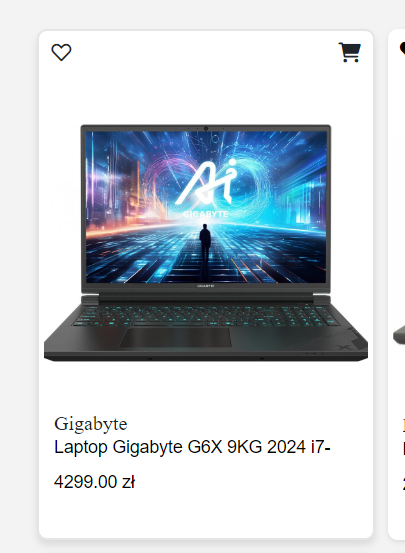
\includegraphics[width=0.5\columnwidth]{images/krzysztofBImages/przyciski-polubienia-koszyka.png}
    \caption{Przyciski polubienia i dodania do koszyka.}
    \label{producs-buttons}
\end{figure}

\begin{figure}[H]
    \centering
    \includegraphics[width=0.5\columnwidth]{images/krzysztofBImages/lista-produktów-respo.png}
    \caption{Wyświetlanie listy produktów - responywność}
    \label{products-respo}
\end{figure}



\subsubsection{Krzysztof Bielkiewicz: Funkcja dodawania produktów do ulubionych}
\label{1.3.14}
\textit{Dodawanie produktów do ulubionych i usuwanie ich z ulubionych przy użyciu django.
Produkt po kliknięciu na przycisk sreca dodaje się do Ulubionych i za poconą skrytu 
JavaScript zmienia ikonke serca na czarne wypełnione. Dane produkty pojawiają się na stronie Ulubione.
Po kliknięciu z powrotem na wypełnione serce produkt usuwa się ulubionych.
Produkty polubione zapisują się w danej sesji i po zalogowaniu są wysyłane do polubień danego usera,
co zapewnia wygode dla użytkownika.}


\subsubsection{Krzysztof Bielkiewicz: Paginacja produktów na stronach}
\label{1.3.15}
\textit{Paginacja dla stron 'Wszystkie produkty', 'Produkty z kategorii', 'Wyszukane produkty', 'Ulubione'.}
\begin{figure}[H]
    \centering
    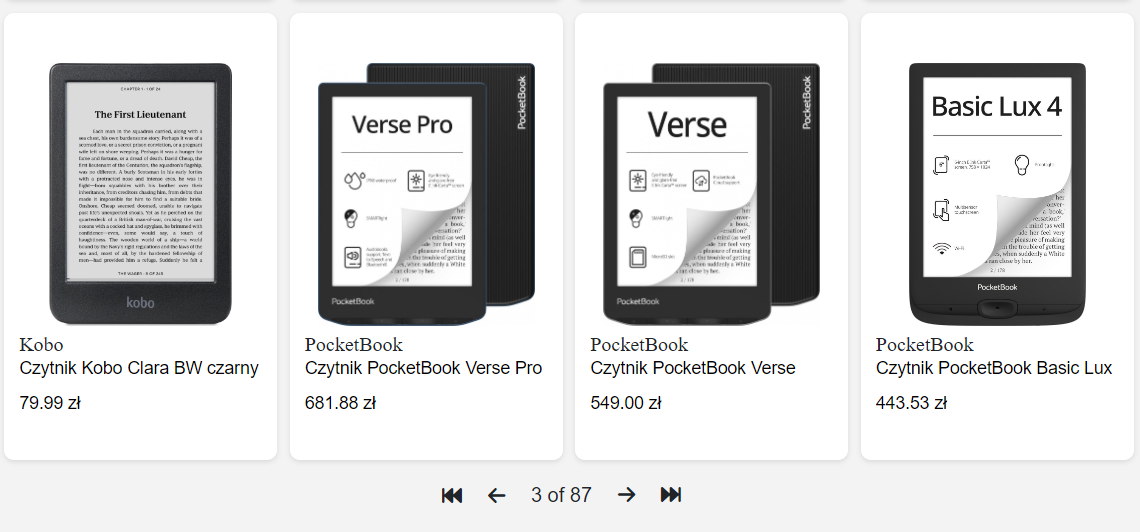
\includegraphics[width=1.0\columnwidth]{images/krzysztofBImages/pagination.png}
    \caption{Paginacja}
    \label{pagination}
\end{figure}


\subsubsection{Krzysztof Bielkiewicz: Oprawa graficzna szczegółów produktu}
\label{1.3.16}
\textit{Oprawa graficzna dla szegółów produktu i jej responywność.}
\begin{figure}[H]
    \centering
    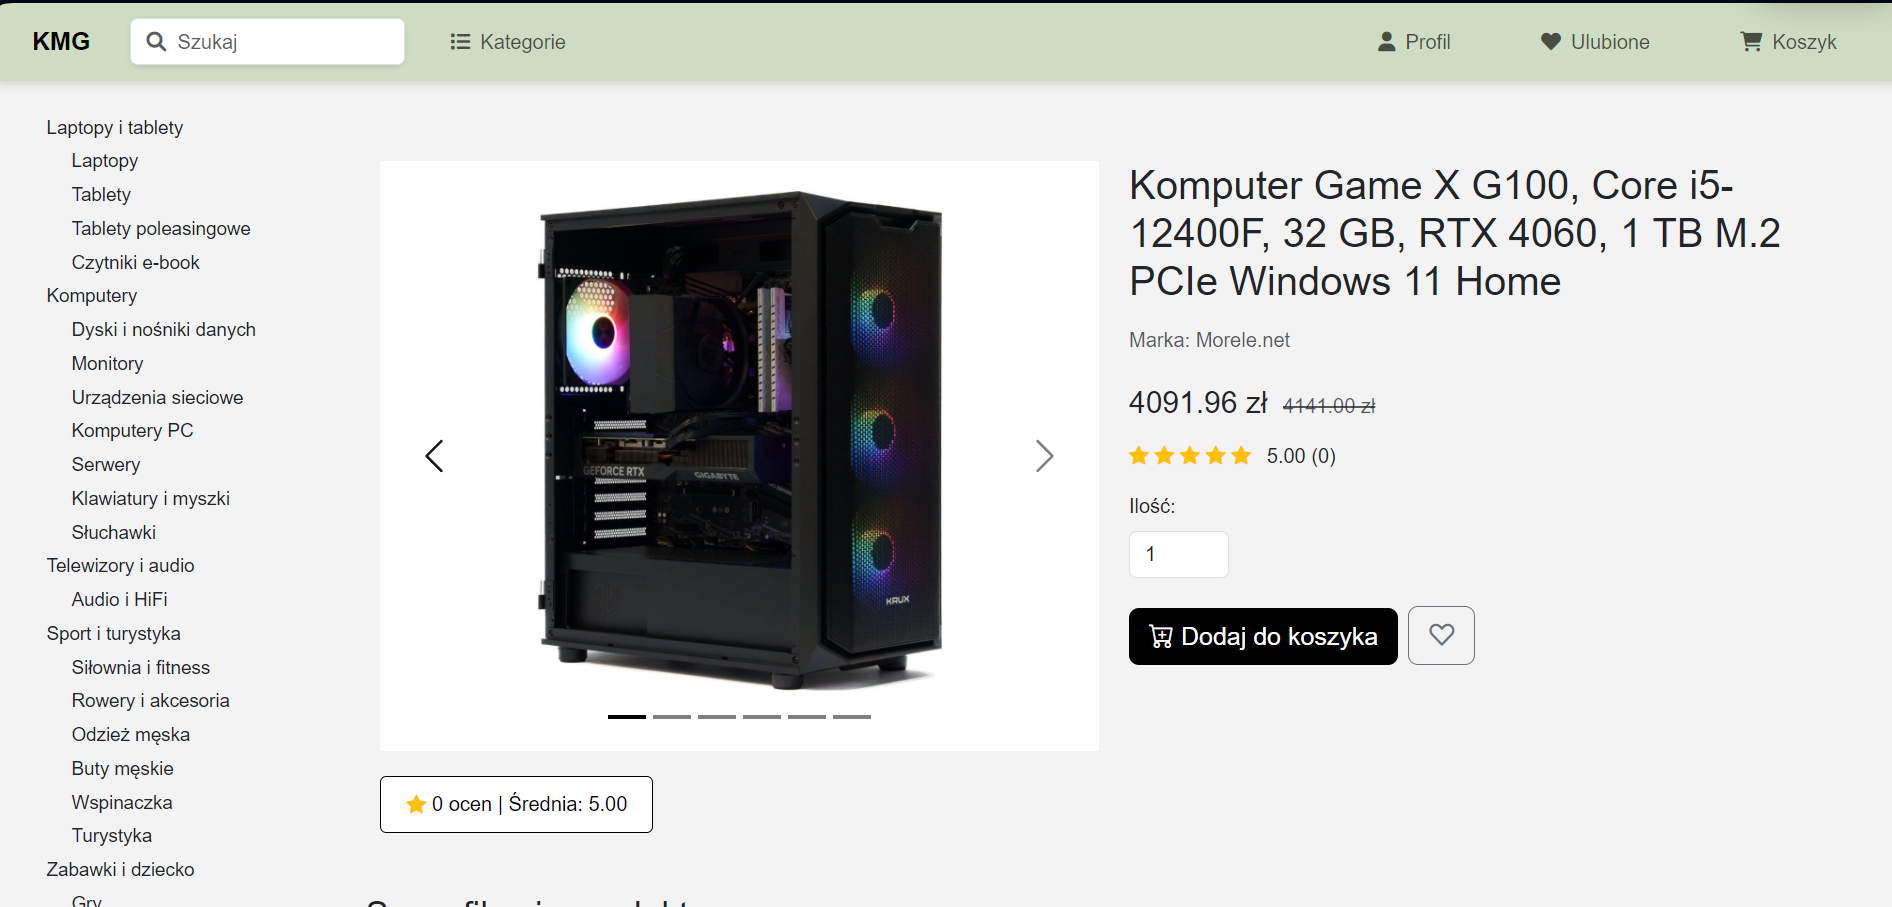
\includegraphics[width=1.0\columnwidth]{images/krzysztofBImages/product-detail.png}
    \caption{Szczegóły produkt}
    \label{product-detail}
\end{figure}
\begin{figure}[H]
    \centering
    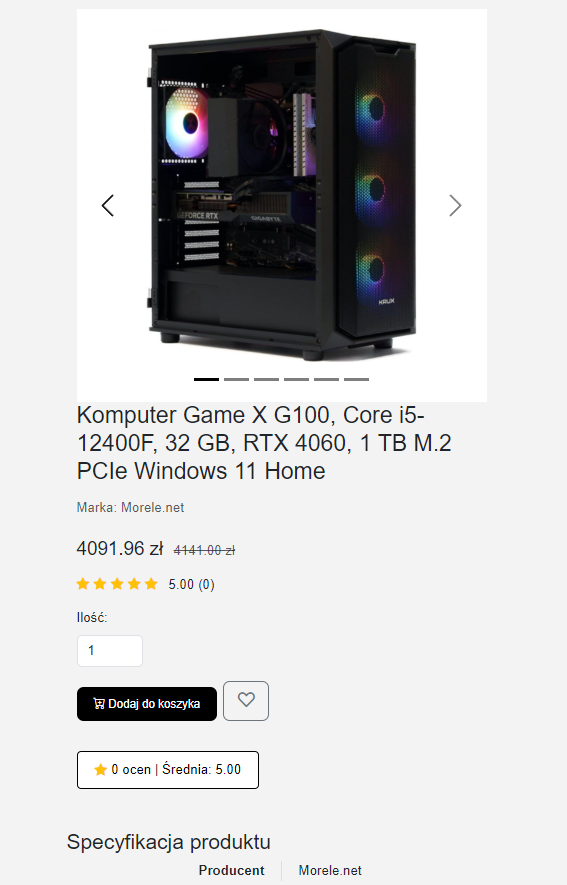
\includegraphics[width=0.5\columnwidth]{images/krzysztofBImages/product-detail-respo.png}
    \caption{Szczegóły produkt - responywna wersja}
    \label{product-detail-respo}
\end{figure}


\subsubsection{Krzysztof Bielkiewicz: Custom errory i oprawa graficzna rejestracji}
\label{1.3.17}
\textit{Własne errory wyświetlające się pod wymaganymi polami,
pole telefonu z automatycznym formatem zrobionym w JS,
 wybór daty urodzenia z zablokowanym wyborem daty w przyszłości (JS). Oprawa graficzna.
 Oraz okienko powiadamiające o udanej rejestracji.}

\begin{figure}[H]
    \centering
    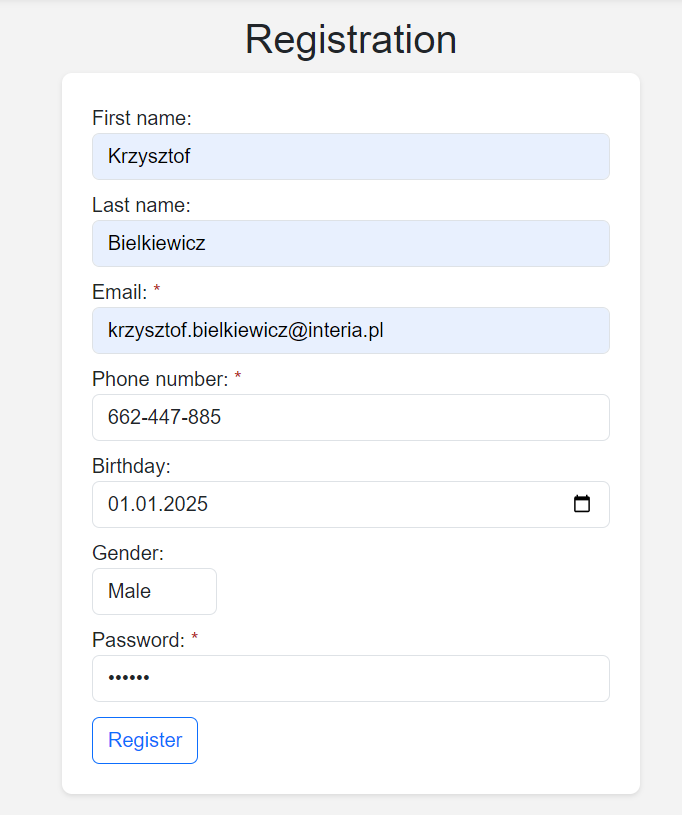
\includegraphics[width=0.5\columnwidth]{images/krzysztofBImages/register-login/registration.png}
    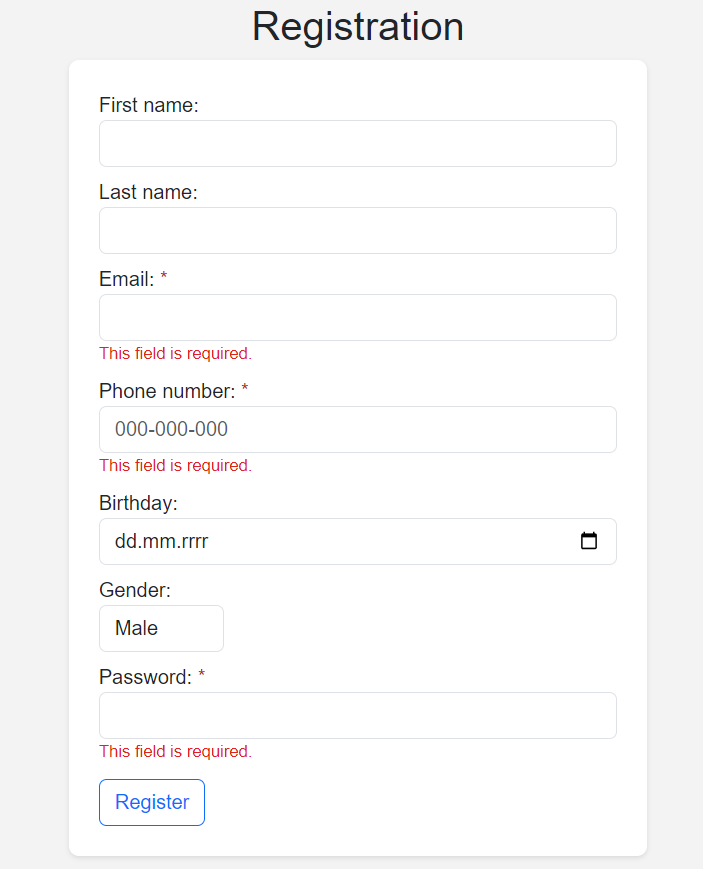
\includegraphics[width=0.48\columnwidth]{images/krzysztofBImages/register-login/register-errors.png}
    \caption{Rejestracja}
    \label{register}
\end{figure}
\begin{figure}[H]
    \centering
    
\includegraphics[width=0.6\columnwidth]{images/krzysztofBImages/register-login/message.png}
    \caption{Powiadomienie}
    \label{message}
\end{figure}


\subsubsection{Krzysztof Bielkiewicz: Custom errory i oprawa graficzna loginu}
\label{1.3.18}
\textit{Oprawa graficzna. Własne errory wyświetlające się pod wymaganymi polami.}

\begin{figure}[H]
    \centering
    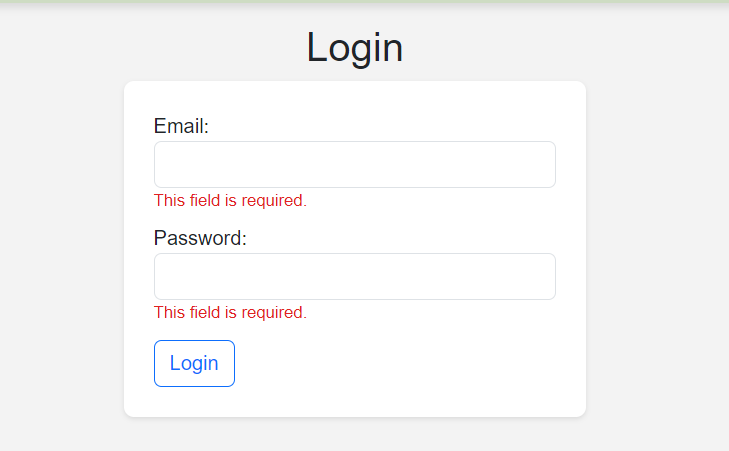
\includegraphics[width=0.8\columnwidth]{images/krzysztofBImages/register-login/login.png}
    \caption{Login}
    \label{login}
\end{figure}


\subsubsection{Karol Woźniak: zadanie nr 1}
\textit{Krótkie wyjaśnienie, opis lub odwołanie do załącznika.}
\subsubsection{Karol Woźniak: zadanie nr 2}
\textit{Krótkie wyjaśnienie, opis lub odwołanie do załącznika.}

\subsection{Załączniki}
\textit{Lista załączników lub dodatkowych materiałów potwierdzających zrealizowane zadania.}

% --------------------------------------------------------------------
%%%%%%% odkomentować gdy bibliografia ma być wewnątrz dokumentu
% --------------------------------------------------------------------
%\begin{thebibliography}{11}
%
%\addcontentsline{toc}{section}{Literatura}
%
%\bibitem{ZAN}
%C. Zannoni and P. Pasini, 
%\emph{Advances in the Computer Simulatons of Liquid Crystals}, Kluwer Academic Publishers, 2000.
%
%\end{thebibliography}

\end{document}

